%% 
%% Copyright 2007, 2008, 2009 Elsevier Ltd
%% 
%% This file is part of the 'Elsarticle Bundle'.
%% ---------------------------------------------
%% 
%% It may be distributed under the conditions of the LaTeX Project Public
%% License, either version 1.2 of this license or (at your option) any
%% later version.  The latest version of this license is in
%%    http://www.latex-project.org/lppl.txt
%% and version 1.2 or later is part of all distributions of LaTeX
%% version 1999/12/01 or later.
%% 
%% The list of all files belonging to the 'Elsarticle Bundle' is
%% given in the file `manifest.txt'.
%% 
%% Template article for Elsevier's document class `elsarticle'
%% with harvard style bibliographic references
%% SP 2008/03/01

%% \documentclass[preprint,12pt,authoryear]{elsarticle}

%% Use the option review to obtain double line spacing
%% \documentclass[authoryear,preprint,review,12pt]{elsarticle}

%% Use the options 1p,twocolumn; 3p; 3p,twocolumn; 5p; or 5p,twocolumn
%% for a journal layout:
%% \documentclass[final,1p,times,authoryear]{elsarticle}
%% \documentclass[final,1p,times,twocolumn,authoryear]{elsarticle}
%% \documentclass[final,3p,times,authoryear]{elsarticle}
%% \documentclass[final,3p,times,twocolumn,authoryear]{elsarticle}
%% \documentclass[final,5p,times,authoryear]{elsarticle}
 \documentclass[final,5p,times,twocolumn,authoryear]{elsarticle}

%% For including figures, graphicx.sty has been loaded in
%% elsarticle.cls. If you prefer to use the old commands
%% please give \usepackage{epsfig}

%% The amssymb package provides various useful mathematical symbols
\usepackage{amssymb}
%% The amsthm package provides extended theorem environments
%% \usepackage{amsthm}

%% The lineno packages adds line numbers. Start line numbering with
%% \begin{linenumbers}, end it with \end{linenumbers}. Or switch it on
%% for the whole article with \linenumbers.
%% \usepackage{lineno}
\usepackage{url}
\usepackage{caption}
\usepackage{float}
\usepackage{multirow}
\usepackage{hyperref}
\usepackage{float}
\usepackage[utf8]{inputenc}
\usepackage{graphicx} 		% Add graphics capabilities
\usepackage{amsmath}  		% Better maths support
\usepackage{natbib}	% bibliography style
\setlength{\bibsep}{0.0pt}
\usepackage{eurosym}
\usepackage{placeins}
\usepackage{makecell}
\usepackage{colortbl}
\usepackage{parskip}
\usepackage{xcolor}
\usepackage{dingbat}
% To fix list things: 
\usepackage{enumitem}
\setitemize{noitemsep,topsep=0pt,parsep=0pt,partopsep=0pt,leftmargin=*}
\usepackage{amssymb}
\renewcommand{\labelitemi}{\tiny$\blacksquare$}


\newcommand*\rot{\rotatebox{90}}

%\usepackage{nopageno}
\usepackage{enumitem}
\newcommand{\nb}[3]{
		{\colorbox{#2}{\bfseries\sffamily\scriptsize\textcolor{white}{#1}}}
		{\textcolor{#2}{\sf\small$\blacktriangleright$\textit{#3}$\blacktriangleleft$}}}
\newcommand{\kv}[1]{\nb{Katrien}{red}{#1}}
\newcommand{\q}[1]{``#1''}
%\setlength{\parindent}{0pt}

\journal{Decision Support Systems }

\begin{document}




\begin{frontmatter}

%% Title, authors and addresses

%% use the tnoteref command within \title for footnotes;
%% use the tnotetext command for theassociated footnote;
%% use the fnref command within \author or \address for footnotes;
%% use the fntext command for theassociated footnote;
%% use the corref command within \author for corresponding author footnotes;
%% use the cortext command for theassociated footnote;
%% use the ead command for the email address,
%% and the form \ead[url] for the home page:
%% \title{Title\tnoteref{label1}}
%% \tnotetext[label1]{}
%% \author{Name\corref{cor1}\fnref{label2}}
%% \ead{email address}
%% \ead[url]{home page}
%% \fntext[label2]{}
%% \cortext[cor1]{}
%% \address{Address\fnref{label3}}
%% \fntext[label3]{}

\title{Which Visualisation Works When? Benefits and Trade-offs of Intuitive, Compact, and Detailed Model Representations in Decision Support Systems for Non-expert Users}

%% use optional labels to link authors explicitly to addresses:
%% \author[label1,label2]{}
%% \address[label1]{}
%% \address[label2]{}

\author[label1]{Francisco Guti\'errez\corref{cor1}}
\ead{francisco.gutierrez@cs.kuleuven.be}
\author[label1]{Tom Broos}
\ead{tom.broos@kuleuven.be}
\author[label1]{Karsten Seipp}
\ead{karsten.seipp@gmail.com}

\author[label2]{Xavier Ochoa}
\ead{xavier@cti.espol.edu.ec}
\author[label1]{Katrien Verbert}
\ead{katrien.verbert@cs.kuleuven.be}

\cortext[cor1]{Corresponding author. Tel.: +32 16 32 82 86; Fax: +32 16 32 79 96.\\E-mail address: francisco.gutierrez@cs.kuleuven.be}
%COMMENT: update telephone number

\address[label1]{Departement Computerwetenschappen, KU Leuven, Leuven, Belgium}
\address[label2]{Escuela Superior Polit\'ecnica del Litoral (ESPOL), Ecuador}


\begin{abstract}
%% Text of abstract

   Researchers have reported a lack of experience and low graph literacy as major problems when making Visual Analytics (VA) available to non-expert users. It therefore is important to understand strengths and weaknesses of different visualisations in the decision-making process of this user group. This paper explores benefits and challenges of an intuitive, a compact, and a detailed visualisation for supporting the analysis in a VA application for non-expert users in two different decision making contexts. In two between-subjects studies (\emph{N} = 210, \emph{N}=271) we find that previously reported challenges can be addressed by matching the type of representation to the degree of insight needed to solve a problem. Whereas the utility of a compact visualisation is limited, an intuitive visualisation works best for easy and medium difficulty tasks, with a detailed visualisation representation being most suitable for hard-level tasks. We suggest an increase of visualisation complexity with an increase in task complexity and we provide recommendations for implementation.

%[COMMENT] I will edit the abstract later
\end{abstract}

\begin{keyword}
%% keywords here, in the form: keyword \sep keyword

%% PACS codes here, in the form: \PACS code \sep code

%% MSC codes here, in the form: \MSC code \sep code
%% or \MSC[2008] code \sep code (2000 is the default)
Visual Analytics \sep Laymen \sep Graph literacy \sep Decision-making
\end{keyword}

\end{frontmatter}

%% \linenumbers

%% main text




\section{Introduction}
% =============================================================================

In our daily lives we may consider multiple risks when planning a financial investment, a project strategy, or when finding a clean and safe place to live. Visual analytics (VA) offers a promising approach to facilitate such decision-making. The core of VA is to support analytic reasoning by interacting with automated and visual data analysis \citep{keim_visual_2008}. By providing control over a variety of settings, users are able to steer complex algorithms. Visualising the results instantly, VA applications gradually support users in their sense-making process, allowing them to gauge the effects of different parameters and to gain more insight with each step of the human-computer dialogue \citep{yi2007toward}. While the interactive steering of algorithms allows insight into large data sets, there still is a need for research concerning the most adequate presentation of such an analysis with regards to a certain group of users \citep{speier2006influence, gettinger2012shall}. An increasing amount of rich data sources (including social data streams and geo-spatial data) is available online to support the decision-making needs of users inexperienced in visualisation and digital analysis (referred to as \emph{non-expert users} in the remainder of this paper). Yet, despite the growing need of this user group to control complex analytical processes, little work has been undertaken to support them \citep{keim2010mastering}. Examples include researchers in the humanities who want to apply analysis techniques to large text corpora \citep{john} and families looking for a place to live. % While these users are experts in their domains, they usually have little expertise on data processing.  %Domain knowledge may influence users in interpreting visualisations \citep{wright_utility_1984} and 
However, such users may have different degrees of ``graph literacy'' that impact their understanding of a certain representation \citep{pinker_theory_1990}. Simple, intuitive visualisations may be easier to understand absolute effects, but abstract ones might offer more detail and insight into the underlying data and processes at the cost of ``representational compatibility'' \citep{sparrow_graphical_1989}. Although a lot of research has been geared towards finding the most suitable representation of different types of data \citep{Wongsuphasawat2016}, researchers report challenges that non-expert users face when using these interactively in VA \citep{huang2015personal,kwon2011visual}. To address this, we need to investigate strengths and weaknesses of different representations to optimally support non-expert users in difficult decisions, such as risk assessment. Our research questions are as follows: 

\emph{1. Regarding criteria such as speed, accuracy, usability, and uncertainty, what are the benefits and challenges of intuitive, detailed, and compact visualisations in an interactive decision-making process?}

\emph{2. How do the visualisations' performance measures accuracy, actions, and time spent relate to task difficulty?}

To answer these research questions, we designed and evaluated two sets of visualisations to support decision making. The first study focuses on evaluating intuitive, compact and detailed representations for the risk-based decision-making process for non-experts in an application facilitating the exploration of quality of life (\emph{QoL}) and \emph{Happiness} in a variety of cities. The second study evaluates intuitive, compact and detailed representations for financial decision making processes for non-expert users. Results of these two user studies indicate that ...

This paper is organised as follows. We first present related work on decision support and visual analytics applications, as well as evaluation metrics to evaluate the utility of such applications. Then, we present two user studies that assess the benefits and drawbacks of intuitive, compact and detailed representations to support decision making.  After answering the research questions, we provide advice for practitioners and academics aiming to build VA applications for non-expert users.

\section{Previous Work} % (fold)
\label{sub:previous_work}
% =============================================================================

%This section will review previous work from the fields of decision support systems and visual analytics, as well as our chosen methods of evaluation. %To simplify the structure, the most relevant work is reviewed separately.


%\subsection{Visual analytics} % (fold)
%\label{sub:visual_analytics}
% =============================================================================
%- overview of topic
%- examples of papers helping solve a problem for domain experts with intuitive / domain-specific viz
%... in different domains
%... keim 2002/2008 areas of VA and its challenges



%>> not clear what works when, how well domain-specific approaches compare to other more abstract approaches

%>> need to know why /what works when, is necessary, helps, is bad, useless etc. wt what type of tasks and step in the sense-making process



%\subsection{Information Visualisation} % (fold)
%\label{sub:informatio}
% =============================================================================
%- graph literacy
%- Data Voyager
%- that journal paper

%>> We know how to PRESENT data, but not how that presentation works in SOLVING a problem! And what the cost/benefit of such a viz in a certain problem case may be



\subsection{Decision Support and Visual Analytics} % (fold)
\label{sub:informatio}
% =============================================================================
%- graph literacy
%- Data Voyager
%- that journal paper

%>> We know how to PRESENT data, but not how that presentation works in SOLVING a problem! And what the cost/benefit of such a viz in a certain problem case may be


%In the Decision Support Systems (DSS) literature, the decision-making process has been modeled as an iterative process of problem recognition, perspective development, perspective synthesis, actions, and results \citep{park2016bicentric}. Visualisation plays a key role, as it facilitates human decision-making by providing structured views of information pertaining to the problem space \citep{shim2002past}. VA combines interaction with traditional information visualisation (IV) techniques with facilities for updating, steering, and improving the analytic processes \citep{keim2010mastering}. It has thus become a well-established method to support decision-making in a wide variety of domains, including health-care and finance \citep{rudolph2009finvis,abidi2001knowledge}. Another domain of growing importance to IV and VA is the domain of digital humanities \citep{jessop2008digital}, which uses computing technologies to facilitate humanities research. Typical examples include timeline visualisation and geographic maps to study the history of philosophical ideas \citep{timemapper}. Pending the nature of the data and context of use, a plethora of visualisation techniques exists. Yet, there is a lack of knowledge regarding the suitability of a particular interactive visualisation in a certain setting for particular users \citep{he2016interactive}. This is, despite the strong impact of choice of representation on the analysis outcome \citep{speier2006influence, gettinger2012shall}. It therefore is important to research which representation works when in a decision-making process, and what the benefits and drawbacks of different approaches may be for the growing group of non-expert users.

In the Decision Support Systems (DSS) literature, the decision-making process has been modeled as an iterative process of problem recognition, perspective development, perspective synthesis, actions, and results \citep{park2016bicentric}. Visualisation plays a key role to support the development of these multiple perspectives. Visualisation facilitates human decision-making by providing structured views about information pertaining to the decision-making problem space \citep{shim2002past}. 

Visualisation is a well-established method to support decision making in a wide variety of domains, including health-care and financial services. \cite{abidi2001knowledge} used multiple visualisation techniques, ranging from graphs to 3D hypercube maps, to support knowledge based decision making in health-care. \cite{tiis} showed that accuracy of recommender systems that suggest relevant items to a user increases with a set-based cluster map representation compared to a traditional ranked list of recommendations. 
\cite{speier2003influence} showed that particularly when the potential solution set is large, visual query interfaces help users with greater effectiveness than text-based interfaces. 

Recent studies show how visualisation affects and supports user decision making in the context of financial services \citep{ben2012assessing}. 
Another area where the role of visualisation to support decision making is increasingly recognised is digital humanities \citep{jessop2008digital}: a research field that comprises the use of computing technologies to facilitate humanities research. Typical examples include timeline visualisation and geographic maps to study the history of philosophical ideas \citep{timemapper}. 

% and a node-link diagram that shows relationships between people \citep{ghoniem2004comparison}. Set-based visualisations focus on representing relationships between clusters or sets. Grouping data elements in sets is a common task in many decision scenarios \citep{riche2010untangling}. For example, when analysing documents, linguists often group words into semantic categories and topics. Similarly, when analysing social networks, sociologists group people into communities and study their relationships. 

The role of interactivity in visualisations has been highlighted in the literature \citep{park2016bicentric}. 
Interaction techniques are increasingly supported in DSS to let users navigate to the data sources of visual analytics. Interactive data visualisations allow users to explore a data set, often by providing details on mouseover, or panning and zooming. Shneiderman's visual information seeking mantra \citep{shneiderman1996} captures the essence of good designs for interactive visualisation: \emph{overview first}, \emph{zoom and filter}, then \emph{details-on-demand}. 
Interactive processes of filtering and visual representation guide not only the analytical process, but also tell a story in a way that conveys useful and actionable insights. An interactive version of self-organizing map visualisations is shown to reduce the cognitive load during Internet browsing tasks \citep{yang2003visualization}.

Pending the nature of the data and use context, many different forms of visualisation and interaction techniques exist. Spence \citep{spence2001information} classified a wide variety of visualisation techniques according to the data dimensions that they visualise. These dimensions refer to the number of attributes that are present in the visualised data. 
Histograms and word clouds are commonly used for one-dimensional data. Scatter plots are the most common representation of two dimensional data. Multivariate data sets are often visualised using parallel coordinates, starplots, or glyph-based techniques. Hierarchical data are often depicted using node-link diagrams, treemaps and sunbursts. 
Whereas the various techniques have been used in several application areas, there is a lack of knowledge which visualisation and interaction techniques work best for particular settings and for particular users \citep{he2016interactive}. In addition, research has shown that the 
 choice of representation of data influences decision-making outcomes \citep{speier2006influence, gettinger2012shall}. Thus, there is a need to research which representations work better in decision-making contexts and what benefits and drawbacks of different approaches are.


In recent years, the importance of Visual Analytics to support decision-making has grown \citep{keim_visual_2008}. Visual analytics extends interaction of traditional information visualisation techniques with facilities for updating, steering and improving the analytic processes. The key objective is to incorporate feedback from end-users to improve an automatic analysis process. 

Interesting examples have been presented at the digital humanities conference in 2015, including an interactive visual analysis of German Poetics \citep{john} that visualises text alignments and focuses on improving current alignment algorithms in an iterative and integrated process. Thus, visualisation is used not merely as a means of presenting the end results of text mining but rather as an analytic approach to data at all points in the text-mining process: from the initial stages of data exploration and hypothesis evaluation, to user-driven feedback for refining text-mining rules and parameters, to generating new hypotheses and questions. This  visual analytics approach has a large potential for future research as it enables to bring human intelligence into the analytic process and to refine previous assumptions and hypotheses on the fly.


Although several interesting prototypes have been developed, little work has been done to enable non-experts in data processing to conduct and steer the analysis \citep{keim2010mastering}. Examples include researchers in the humanities who want to apply analysis techniques to large text corpora, or teachers who want to analyse student data. While these users are experts in their domains, they usually have little expertise on data processing. To support decision-making,  the notion of data quality and the confidence of the analysis algorithm need to be appropriately represented.  This lack of skills leads to a common pattern where the analytical task is shared by two user roles \citep{bernard2012visual}: in a first step, the domain expert but non data-processing expert (e.g. a humanities scholar or teacher) defines criteria for useful data and requirements for the analysis. In a second step, a data-processing expert -- usually ignorant of the domain -- is responsible to choose, modify and integrate automatic and visual analysis methods. Whereas such an approach is feasible and has resulted in several interesting prototypes that can be used by non-technical users, for instance to analyse risk and uncertainty in financial data \citep{rudolph2009finvis}, it is also constrained by several limitations.

The main issue with the decoupling of the data-processing design and the data-processing use is that vital information to understand the analysis is lost in the visual translation. The most pernicious omission in this translation is the suppression of data uncertainty and quality information. Dealing with uncertainty and trust in visual analytics is non-trivial because of the large amount of noise and missing values originating from heterogeneous data sources and bias introduced by automatic analysis methods as well as human perception \citep{thomas2009challenges}. To face this problem, the notion of data quality and the confidence of the analysis algorithm need to be appropriately represented. The analysts need to be aware of the uncertainty and be able to analyse quality properties at any stage of the data analysis process. Whereas several approaches have been researched under the umbrella of ‘data wrangling’ \citep{kandel2011research}, most of this work concentrates on preprocessing of data (i.e. data entry, data (re)formatting, data cleaning, etc.). Little work has been done to represent data quality and confidence in parallel to visualisation of outcomes of the analysis. Such visualisation is vital to support decision-making: as what constitutes an error is often context-dependent and requires human judgment of domain experts \citep{kandel2012profiler}, there is a need to research how such variables can be represented in parallel to outcomes of an iterative analysis process. In this paper, we focus specifically on the design and evaluation of different visualisations that represent these variables for non-expert users. In two elaborate user studies, we evaluate different aspects of the utility and effectiveness of different designs. We discuss relevant evaluation metrics in the next section. 

%zhang2016prediction
%Theoretically, uncertainty exists in all predictions [30]. Since CF techniques compute predictions based on the models that are heuristic approximations of human processes and the data that are extremely sparse and incomplete [22], the predictions may occasionally be severely biased. Meanwhile, it has been empirically shown that a recommendation agent’s system quality, including prediction uncertainty, has significant effects on users’ decision making satisfaction [4]. Therefore, addressing the prediction uncertainty in CF should be of considerable research value.
%Despite the sizeable body of research on recommender systems and various approaches that try to improve the overall prediction accuracy of CF-based recommendation algorithm, there is much less attention paid to the uncertainty of each individual prediction. In particular, each prediction generated by CF should not be treated equally and its uncertainty should be carefully modeled by considering the CF predictive process. This gives us a new direction to improve the personalized ranking accuracy. Serving as a postprocessing strategy, our new ranking approach can be applied after the CF algorithms have generated predictions. Thus, the main contribution of this work is that it offers a novel angle for the improvement of ranking accuracy after applying any CF algorithm.


%ribeiro1995uncertainty
%Many decisions involve uncertainty, yet most decision support systems (DSSs) and expert systems (ESs) are poorly equipped to deal with such problems. This paper employs an abductive perspective to propose a prototype framework for tackling uncertainty handling in DSS and ES. Five major features of such a framework, a user-friendly dialogue, a case-base, a knowledge-base, approximate reasoning and a fuzzification/defuzzification mechanism are presented and developed. These are supported by an extended example.

%example VA in supply network %park2016visual
%Grounded in cognitive fit theory, we demonstrate that an interactive visual system that dynamically adjusts visual representations to the decision environment can significantly enhance decision-making processes in a supply network setting. 

% from JVLA
%A limitation of the discussed studies may be that the majority appears to focus on experts (despite a few exceptions including laymen) and that they use relatively small numbers of participants \cite{maceachren_visualizing_2005}. Such a limitation may not come as a surprise, as recruiting experts can be difficult. But with the increasing use of information visualisation and Visual Analytics in consumer applications, it appears worthwhile to explore whether the findings of previous work regarding the performance of certain visual means to represent uncertainty to (mostly) experts, may also be applicable to laymen. A lot of work has focussed on visualisations that include a geographic component -- such as the spatial distribution of data. It therefore seems suggestive to explore whether the findings for representing uncertainty in GV may not also be applicable to other domains dealing with areal uncertainty. Especially the visualisation of algorithms that use the distance to an ideal classification point (such as a the centroid of a K-means cluster or the trend line of a linear regression) as a way to describe the degree of certainty with which a data point may belong to a particular class or correspond to an ideal model, could be a worthwhile field of exploration. An application to this domain seems important, as such algorithms may be used in Visual Analytics applications that are to help users gain insight into complex coherences. To make a good decision, it may be necessary to offer a high degree of depth and complexity by visualising the data and its position in the classification space generated by the underlying algorithm. This prompts an investigation of the question whether knowledge from the domain of geovisualisation and cartography may not be transferable to the domain of algorithm visualisation. As both may deal with areal uncertainty, such a transfer may help users verify the reliability of a classification or prediction to make a more informed decision.


%In recent years, the importance of VA to support decision-making has grown \citep{keim_visual_2008}. Visual analytics extends interaction of traditional information visualisation techniques with facilities for updating, steering and improving the analytic processes. %The key objective is to incorporate feedback from end-users to improve an automatic analysis process. 

%Interesting examples have been presented at the digital humanities conference in 2015, including an interactive visual analysis of German Poetics \citep{john} that visualises text alignments and focuses on improving current alignment algorithms in an iterative and integrated process. Thus, visualisation is used not merely as a means of presenting the end results of text mining but rather as an analytic approach to data at all points in the text-mining process: from the initial stages of data exploration and hypothesis evaluation, to user-driven feedback for refining text-mining rules and parameters, to generating new hypotheses and questions. This  visual analytics approach has a large potential for future research as it enables to bring human intelligence into the analytic process and to refine previous assumptions and hypotheses on the fly.


%Although several interesting prototypes have been developed, little work has been done to enable non-experts in data processing to conduct and steer the analysis \citep{keim2010mastering}. Examples include researchers in the humanities who want to apply analysis techniques to large text corpora, or teachers who want to analyse student data. While these users are experts in their domains, they usually have little expertise on data processing. %To support decision-making,  the notion of data quality and the confidence of the analysis algorithm need to be appropriately represented.  %This lack of skills leads to a common pattern where the analytical task is shared by two user roles \citep{bernard2012visual}: in a first step, the domain expert but non data-processing expert (e.g. a humanities scholar or teacher) defines criteria for useful data and requirements for the analysis. In a second step, a data-processing expert -- usually ignorant of the domain -- is responsible to choose, modify and integrate automatic and visual analysis methods. % Whereas such an approach is feasible and has resulted in several interesting prototypes that can be used by non-technical users, for instance to analyse risk and uncertainty in financial data \citep{rudolph2009finvis}, it is also constrained by several limitations.

%The main issue with the decoupling of the data-processing design and the data-processing use is that vital information to understand the analysis is lost in the visual translation. The most pernicious omission in this translation is the suppression of data uncertainty and quality information. Dealing with uncertainty and trust in visual analytics is non-trivial because of the large amount of noise and missing values originating from heterogeneous data sources and bias introduced by automatic analysis methods as well as human perception \citep{thomas2009challenges}. To face this problem, the notion of data quality and the confidence of the analysis algorithm need to be appropriately represented. The analysts need to be aware of the uncertainty and be able to analyse quality properties at any stage of the data analysis process. Whereas several approaches have been researched under the umbrella of ‘data wrangling’ \citep{kandel2011research}, most of this work concentrates on preprocessing of data (i.e. data entry, data (re)formatting, data cleaning, etc.). Little work has been done to represent data quality and confidence in parallel to visualisation of outcomes of the analysis. Such visualisation is vital to support decision-making: as what constitutes an error is often context-dependent and requires human judgment of domain experts \citep{kandel2012profiler}, there is a need to research how such variables can be represented in parallel to outcomes of an iterative analysis process.
%Visualiszing data and process quality to support decision-making is not a topic that has been explored extensively in the visualiszation literature \citep{kennedy2013visual}. There has been research into specific techniques for uncertainty visualiszation \citep{sanyal2009user} and what uncertainty itself entails \citep{skeels2010revealing}, but it tends to concentrate on preprocessing data before such data is used in applications \citep{kandel2011research}, rather than looking at how to communicate quality indicators to support decision-making by domain experts. 




\subsection{Evaluation metrics} % (fold)
\label{sub:evaluation_metrics}
% =============================================================================


Metrics to evaluate VA applications comprise a variety of criteria. However, definitive, generalisable guidelines do not appear to exist. We therefore analysed previous work to define a set of metrics that may be considered useful in gauging an application's adequacy for supporting the user's decision-making process on the most important levels.

\cite{laskowski_framework_2007} provide an overview of the measures applied by judges of the Visual Analytics Science and Technology visualisation contest. They recommend considering correctness of the analysis, degree of decision support, and efficiency of operation. \cite{lex_caleydo:_2010} consider confusion, readability, information salience, time spent, accuracy, and domain-specific measures. In addition, \cite{wang_two-stage_2011} recommend the inclusion of a set of qualitative criteria based on the work of \cite{scholtz_beyond_2006}: Situational awareness, collaboration, interaction, creativity, and utility. A different approach is taken by  \cite{hearst_evaluating_2016} who combine heuristic evaluation and question-based scoring. \cite{yang_understand_2014} evaluate information graphics based on user preference and their capability to provide different levels of insight. While they could establish a link between information type and presentation, similar to  \cite{Wongsuphasawat2016}, they did not investigate how well the representations would perform as part of an interactive analysis in a VA application. \cite{isenberg_systematic_2013} review evaluation practices in the visualisation community and list adequacy of representation, support for collaboration, user performance and experience, and qualitative feedback as popular criteria. Yet, not all measure might apply for all applications.

As gaining insight is a key factor, it seems suggestive to explore an application's suitability for achieving different levels of insight using a set of metrics introduced by previous work. Although controlled experiments may be inadequate \citep{Perer:2008:ISV:1357054.1357101} for comprehensively evaluating a VA application, we decided to employ this technique as we intended to define general, quantifiable aspects of different representations, rather than evaluating the application as a whole. We therefore focused on transferable properties, not limited to a specific context, organized as follows:

Metrics to evaluate user performance on each visualisation for each level of difficulty of tasks:

\begin{itemize}
  \item \textbf{Accuracy}: Does the visualisation help to improve the precision of participants when solving the tasks?
  \item \textbf{Actions} : How many actions are required with the visualisation to solve the tasks?
  \item \textbf{Time Spent}: How quickly can a user interpret the visualisation to solve the task?  
\end{itemize}

Subjective feedback from the participants about their attitudes towards usability aspects of visualisations:

\begin{itemize}
  \item \textbf{Visual Appeal}: Are the visualisations appealing to the participants?
  \item \textbf{Ease of use}: Is the visualisation facilitating the solve of tasks?
  \item \textbf{Suitability}: How do the participants perceive the visualisation when solving the tasks in the given context? 
  \item \textbf{Liked it}: Do the participants like the visualisation in general?
  \item \textbf{Task Difficulty}: Does the visualisation make the tasks look easier or harder than they are?
\end{itemize}

Subjective feedback from the participants about their attitudes towards uncertainty aspects from the visualisations:

\begin{itemize}  
  \item \textbf{Trust}: Do the participants trust what they see depicted in the visualisation?
  \item \textbf{Confidence}: Do the participants feel confident with their responses when using the provided visualisation?
  \item \textbf{Credibility}: Do the participants believe in what is depicted in the visualisation?
  \item \textbf{Understanding}: Is the communication of uncertainty in the visualisation easy to understand?
  \item \textbf{Accuracy representation}: Is the representation of the accuracy adequate for the problem at hand?
\end{itemize}

The performance of the different visualisations with regards to these aspects is to be determined from a set of tasks. These consist of a mixture of confirmatory and exploratory questions and are separated into three different levels of difficulty. We thereby expect to achieve an understanding of the strengths and weaknesses of representing model predictions using either intuitive, compact, or detailed visualisations in response to user input. 

\section{Study 1: Quality of Life and Happiness}
\subsection{Design Motivation} % (fold)
\label{sec:design_motivation}
% =============================================================================


% A goal of VA is to support domain experts in the decision-making process, who lack data processing skills. As domain experts are difficult to recruit in large numbers, we decided to situate our study in a domain in which most people may be considered ``experts'': 

Non-expert users of VA applications face a lot of challenges, (e.g. support people with limited visualization
literacy and VA experience, fit into personal life routines and physical surroundings, apply appropriate baselines to support reasoning about data) \citep{kwon2011visual,huang2015personal}. With the rise of \q{Personal Visual Analytics} (PVA), it has become important to explore how application designers may overcome these and support non-experts in the decision-making process. A possible application is the search for a place to live. Such a task may be a major life decision that requires careful assessment of risks and benefits. As this may be difficult and laborious, we chose this scenario as the basis of our study to evaluate three different model representations in the decision-making process of non-experts:

\noindent \textbf{What and Where: Intuitive Representation}.
Finding a place to live is factual and emotional. Basic emotions are frequently perceived via a person's face. As users would typically be looking for a place with a high quality of life where they can be happy, we encoded these factors into Chernoff faces \citep{chernoff_use_1973} for a set of cities. By mapping the emotional factors \emph{Happiness} and \emph{Quality of Life} (QoL) to facial expressions, we estimated this visualisation to have a high ``representational compatibility'' \citep{sparrow_graphical_1989} and to be particularly suited for answering simple questions concerning aspects of \emph{What} and \emph{Where}.

% We added a numerical readout for \emph{Happiness} and a range-based indicator of uncertainty to offer the same features as the other visualisations in our study.

 % such as changes in size and shape of the head, eyes, nose, and mouth. To address this problem, we only used the eyes and mouth and only used three levels (low, medium, high) mapped to certain value ranges (see section \ref{sub:interaction}). \emph{Happiness} was encoded using the mouth, \emph{Quality of Life (QoL)} using the eyes. 




\noindent \textbf{Why: Detailed Representation}.
The detailed visualisation of a computational model allows users to investigate \emph{Why} a prediction was made. By inspecting the distribution of instances in the classification space and their distance to the model, users can understand the model's ``goodness of fit'' as well as the reasons for potential uncertainty. Differences between the distributions of various risk factors can be depicted simultaneously and effects and interactions understood. However, this is accompanied by a higher cognitive load and requires a certain degree of graph literacy \citep{pinker_theory_1990}. In addition, the scale of the visualisation can influence users in their interpretation \citep{cleveland_variables_1982}. Therefore, it is important to investigate whether the benefits outweigh the potential disadvantages when employed in a risk assessment process for non-expert users.


\noindent \textbf{How: Compact Representation}.
A compact model visualisation provides a close-up, allowing users to examine \emph{How} data are distributed. It provides focused insight into a particular risk, clearly showing its spread and model uncertainty. Yet, providing detail for a single factor comes at the price of depicting relationships between multiple factors. We thus need to explore the benefits and challenges of such a visualisation in a risk-assessment application, and whether this trade-off is beneficial to the decision-making process. As a basis for this visualisation we chose the work of \cite{kay_when_2016} who could demonstrate its usability and precision. However, it is unclear how well it scales to more complex problems.

\noindent \textbf{Uncertainty}. % (fold)
\label{sub:uncertainty}
The visualisation of uncertainty is important to correctly interpret an algorithm's prediction \cite{skeels2010revealing}. \cite{kinkeldey_how_2014} provide a comprehensive overview of the performance of different visual means to represent uncertainty in the domain go Geospatial Visualisation. Although no clear champion appears to exist, altering an element's opacity or lightness of colour seems to be a suitable approach. In accordance with the work of \citep{davis_modelling_1997}, we chose a change in opacity to represent this aspect across the three visualisations. 

% To investigate which visualisation works best for what degree of insight, we kept the interactive component of our VA application consistent, but changed the representation of the resulting prediction to one of the above visualisations, resulting in three applications.
 % that employ the same means of control, but differ in the presentation of the result.

% OR

% To really gain insight into what works when, we keep the control mechanism the same, but changed the representation of the prediction output to one of the three visualisations.

% What works when especially in risk-based decision making
% Risk: Mayor life decision: looking for place to live!!

% section design_motivation (end)

% To investigate which visualisation works best for what degree of insight, we kept the interactive component of our VA application consistent, but changed the representation of the resulting prediction to one of the above visualisations, resulting in three applications.
 % that employ the same means of control, but differ in the presentation of the result.

% OR

% To really gain insight into what works when, we keep the control mechanism the same, but changed the representation of the prediction output to one of the three visualisations.

% What works when especially in risk-based decision making
% Risk: Mayor life decision: looking for place to live!!

% section design_motivation (end)

% section design (end)

\begin{figure}
\centering
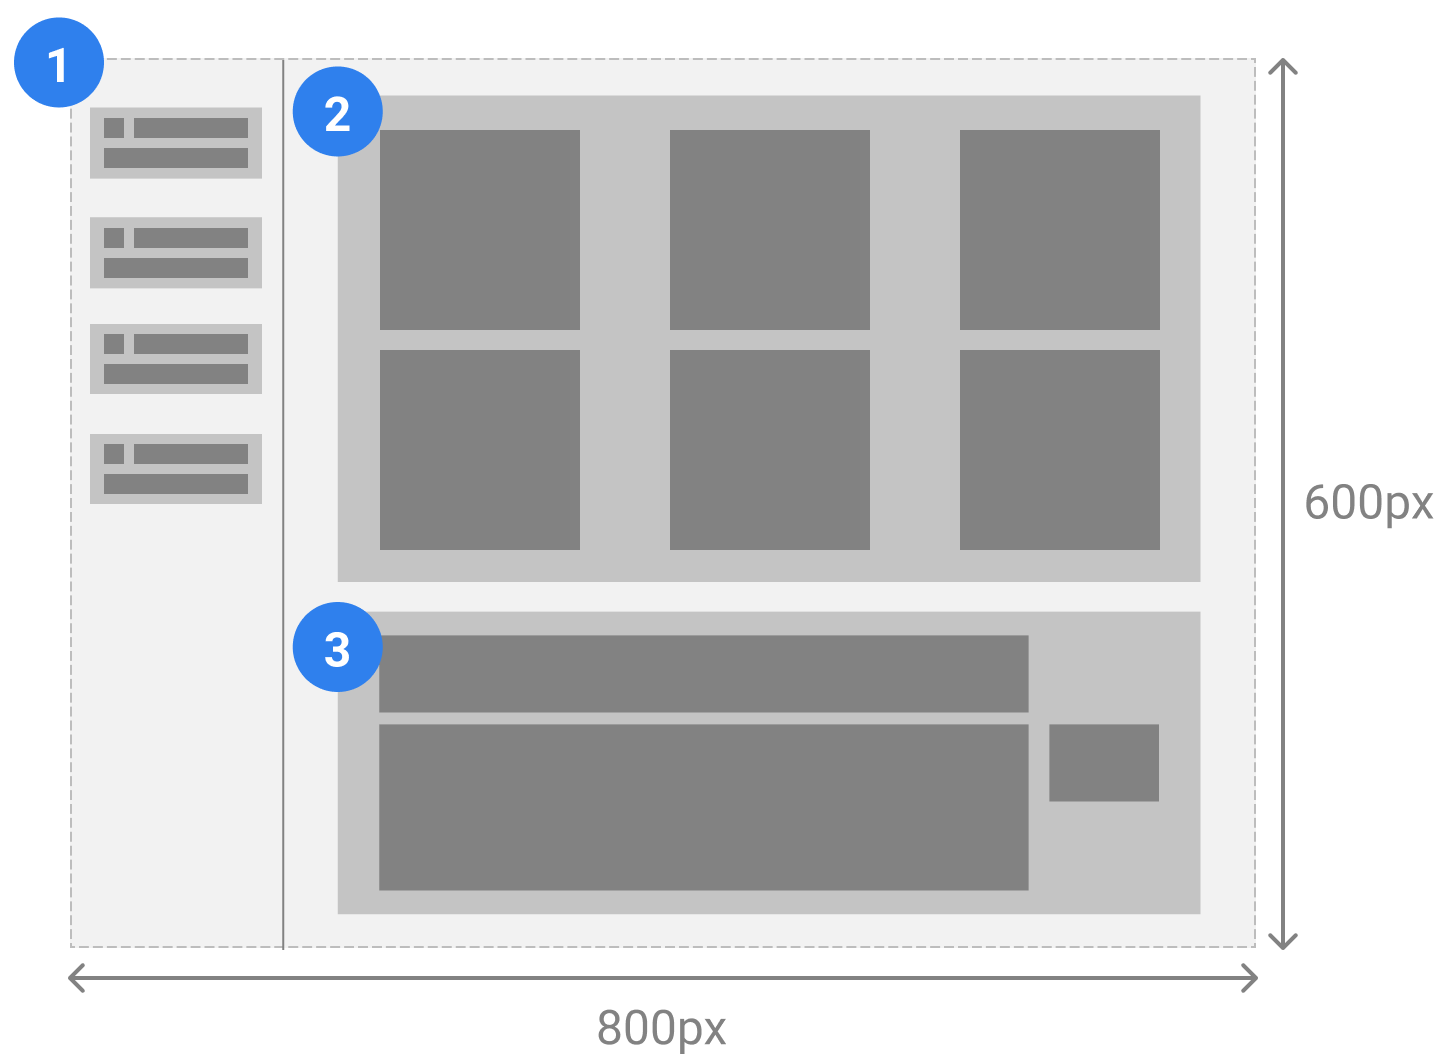
\includegraphics[width=0.75\columnwidth]{figures/whole-app-steps.png}
\caption{The main layout for the three applications in the first and second study. \textbf{(1) The settings section} that shows the controls (i.e. checkbox and sliders) for weighting the variables in the predictions. \textbf{(2) The visualisation section} were the six prediction visualisations were shown. \textbf{(3) Questions section} where users saw the questions they had to answer by interacting with the controls and visualisations.}\label{controls-dots-all}
\end{figure}


\subsection{Application Design} % (fold)
\label{sec:design}

We implemented the visualisations into three Web Applications, one application per visualisation. While prediction algorithm, interaction, and data were the same for all applications, they differed in the visualisation of the predicted outcome. The main layout of the application is shown in Figure \ref{controls-dots-all}. The common modules were as follows:

\subsubsection{Data} % (fold)
\label{sub:data}

We collected data using the Twitter Streaming API to track opinions about different ``risks'' impacting the \emph{QoL} in six U.S. cities: weather, traffic, air quality, and safety. Our architecture supported real-time sentiment analysis using the natural language processing library Pattern by Clips\footnote{http://www.clips.ua.ac.be/pattern}, determining \emph{Happiness} based on the polarity with a score between 0 to 1 (very negative, very positive). We used third-party APIs (Numbeo, AQICN, Yahoo Weather, Bing Traffic API, and others) to measure the real-time opinion on each factor's \emph{QoL}. A prediction was built using a  regression model, training the model with every tweet from the stream. However, to ensure consistency in the visualisations and the conditions, we decided to ``freeze'' the data in a database.
% subsection data (end)


\subsubsection{Model} % (fold)
\label{sub:prediction}


Our regression model used a \emph{QoL} index defined by a set of \emph{QoL} factors in a given city to predict the happiness.
%\vspace{-0.1cm}
%\[Happiness =  \alpha  + \beta  \times  \emph{QoL},\vspace{-0.1cm}\]
%where  \( \alpha \) and \(  \beta \) are the regression coefficients. 
Users could adjust the factors using a set of sliders (Figure \ref{controls-dots-all}). Based on the position of the sliders, a weighting factor is calculated to generate the \emph{QoL} index.
%Let \begin{math} \tau _{f}\end{math} be the set of factors that is selected by the user. The predicted value \begin{math} \widehat{p}\end{math} is computed as \vspace{-0.1cm} \[ \widehat{p}=\frac{\sum_{f\epsilon \tau _{f}}(w_{f}.m_{f})}{\sum_{f\epsilon \tau _{f}}w_{f}}\vspace{-0.15cm} \] with \begin{math} m_{f}\end{math} the mean value between all points of the particular factor \begin{math} f \end{math} and \begin{math} w_{f}\end{math} the importance assigned to this factor by the user with the respective slider. 
Using the \emph{QoL} index, our model predicts people's (\emph{Happiness}) in the given city.
% In general our regression models showed a positive relationship between the \emph{QoL} and \emph{Happiness}, indicating that when quality of life is better people tend to express more happy thoughts on Twitter.

% Francisco to review this. Is this correct? 

% Taking into account the factors selected by the user, a simple linear model is built to predict the \emph{Happiness} and corresponding \emph{QoL}. While \emph{Happiness} is calculated as the mean distance between all points of the active factors, \emph{QoL} results from mapping the calculated point on the regression line to a position on the X-axis, which represents the corresponding value of the \emph{QoL} of the active factors' distributions (Fig. \ref{2-vis}, left). The regression is built using the \emph{lm} package of \emph{R} while the prediction is made using the \emph{predict.lm} package. Based on the ``importance'' setting of the sliders corresponding to the four factors a weighting factor is introduced affecting the horizontal position of the predicted value on the regression line using the following formula.



% Let \begin{math} \tau _{f}\end{math} be the set of
% factors that is selected by the user. The predicted value \begin{math} \widehat{p}\end{math} is
% computed as:

% \[
% \widehat{p}=\frac{\sum_{f\epsilon \tau _{f}}(w_{f}.m_{f})}{\sum_{f\epsilon \tau _{f}}w_{f}}
% \]

% with \begin{math} m_{f}\end{math} the mean value between all points of the particular factor  \begin{math} f \end{math} and \begin{math} w_{f}\end{math} the importance assigned by the user to this factor. 

%The weight of each factor can be determined by the user as described in the following section.

% subsection prediction (end)


\subsubsection{Interaction} % (fold)
\label{sub:interaction}
Each application showed the four risks determining \emph{Happiness} and \emph{QoL} on the left side of the screen (Fig. \ref{controls-dots-all}, left). Below these was a key describing how to interpret the model's uncertainty in the visualisation. Each risk could be activated/deactivated via a checkbox and its weighting in the prediction could be adjusted via a slider from 0\% (not important, but still considered) to 100\% (very important). Influencing the prediction works as follows: The user activates the risks of interest and moves the sliders. The prediction is updated immediately using the new weighting and the results regarding \emph{Happiness} and \emph{QoL} shown in the visualisation. 
% This way the user can gain insight and understanding into the risks' impact.
% on these aspects.
% subsection interaction (end)

\begin{figure*}
\centering
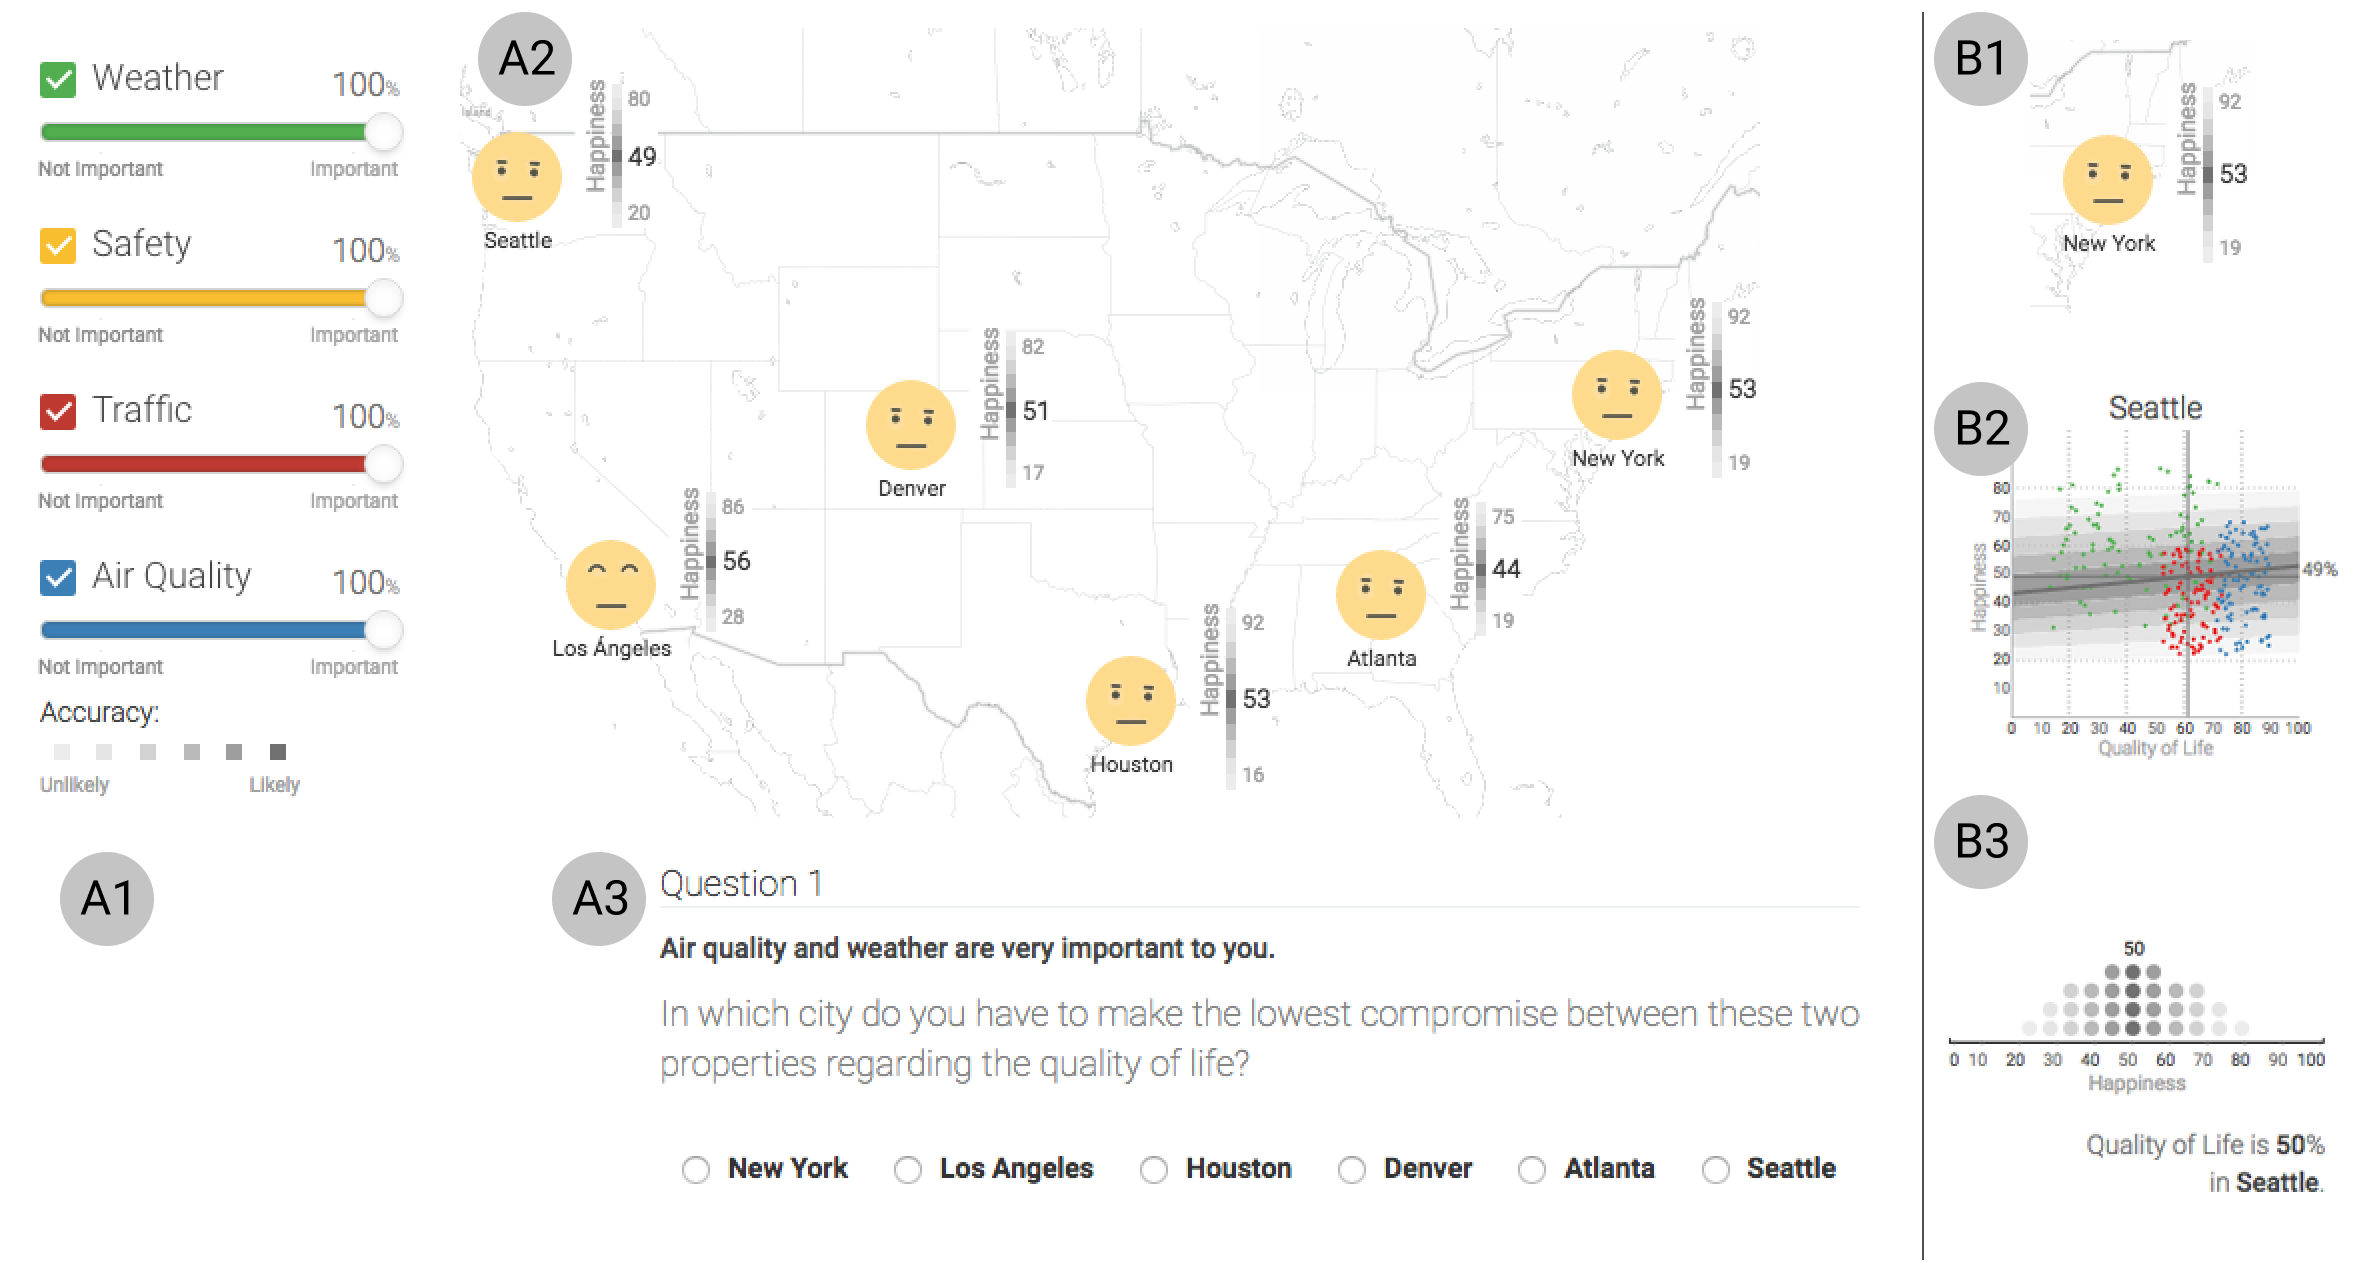
\includegraphics[width=\textwidth]{figures/whole_app1.png}
\caption{\textbf{A) Left:} Screen shot of the main screen in the application. \textbf{A1.} \textbf{Settings section}, where users selected the values for the prediction variables. \textbf{A2.} \textbf{Visualisations section}, where the predictions were shown. \textbf{A3.} \textbf{Questions Section}, where users had to select the correct answer. \textbf{B) Right:} The three different visualisations used to represent the predictions. \textbf{B1.} \textbf{Intuitive} visualisation. \textbf{B2.} \textbf{Detailed} visualisation. \textbf{B3.} \textbf{Compact} visualisation.}\label{2-vis}
\end{figure*}


\subsubsection{Visualisation} % (fold)
\label{sub:visualisation}

The prediction model was visualised in the visualisation section of the application \ref{controls-dots-all} using one of the three representations:

\noindent \textbf{Figure \ref{2-vis}, B1: intuitive representation (\emph{map})}. In this condition, the results of the prediction regarding \emph{Happiness} and the corresponding \emph{QoL} of all active risks were displayed using a Chernoff face \citep{chernoff_use_1973}. As these are serially processed \citep{morris2000experimental} and can be slow to interpret \citep{umanath_multiattribute_1994}, we only showed the two relevant variables in three levels, corresponding to a range in which the predicted value resided: Low (0-30\%, medium (31-60\%), high ($>$ 60\%)). Although potentially imprecise, this decision was made to maintain the simplicity and intuitiveness of the visualisation. The actual value of the predicted degree of \emph{Happiness} and the uncertainty of the prediction were depicted on a separate scale next of the face. A tall scale meant a high spread of opinions, a short scale a low one. At the point of the prediction the scale was black, with surrounding values represented by changes in opacity, based on the degree of uncertainty. \emph{QoL} was mapped to the eyes while \emph{Happiness} was mapped to the mouth. Using an intrinsic display of uncertainty by altering the degree of opacity of the faces was also considered, but discarded in favour of consistency with the \emph{Charts} and \emph{Dots} visualisation. Colour palette and level of detail were reduced to a minimum, while all actions like zooming and panning were disabled. 

\noindent \textbf{Figure \ref{2-vis}, B2: detailed representation (\emph{scatter plot})}: This consisted of six coordinate systems (one per city) describing the model built from the distributions of the active risks. The spread of \emph{QoL} of a risk was mapped to the X-axis, the corresponding distribution of tweets describing users' opinion (\emph{Happiness}) of this risk to the Y-axis and then plotted into the coordinate system. The predicted value for \emph{Happiness} was written in text next to the visualisation at the Y-coordinate of the corresponding point of the regression line. The \emph{QoL} that corresponded to the predicted level of \emph{Happiness} could be read from the corresponding point on the X-axis.


\noindent \textbf{Figure  \ref{2-vis}, B3: compact representation (\emph{dot plot})}. This consisted of six visualisations (one per city) showing the posterior distribution of the prediction (\emph{Happiness}), given the selection of the city factors. The most likely predicted value was shown above the mean of the distribution, while the corresponding \emph{QoL} was displayed below the visualisation together with the city name. This visualisation was based on the work of  \cite{kay_when_2016}. Uncertainty was represented using probability and we included a change of opacity (more precisely \q{colour lightness}), which has been shown to be an effective visual variable for this aspect \citep{davis_modelling_1997}. It was mapped to represent the quantiles, by five levels, each corresponding to an increase of 20\%, with the opacity of the visualisation reduced accordingly. Although not a detailed representation, it may nonetheless suffice to judge the prediction's accuracy. Being intrinsic to this visualisation \citep{kay_when_2016}, it served as guide for showing uncertainty in the visualisations \emph{Charts} and \emph{Map}.


% subsection visualisation (end)


\subsection{Preliminary study} % (fold)
\label{sec:preliminary_study}
% =============================================================================
Guided by previous work aiming to evaluate VA applications \citep{laskowski_framework_2007,hearst_evaluating_2016}, three researchers analysed the data and visualisations to form a total of 41 possible questions, comprising the finding of facts, trends, and relationships. These were implemented into three applications and given to six non-expert users (6M, mean age: 29 years, SD: 4.3). Participants answered each question using all three visualisations and rated their difficulty on a five-point Likert scale. Task order was randomised and the study counterbalanced by visualisation.

In many cases, difficulties were rated similarly. We focussed on these and selected three tasks per level of difficulty with a similar rating across all three conditions, ending up with the same nine tasks for all three applications. We then assigned different difficulty levels, following the example of \cite{yang_understand_2014}

\begin{itemize}
  
  \item \textbf{Easy:} Users can answer this question by only operating a single slider to gauge its effect.
  \item \textbf{Medium:} Users can answer this question by operating two sliders and they have to explore their interactions in one city or two cities.
  \item \textbf{Hard:} Users can answer this question by operating at least two sliders and they have to explore their interactions in more than two relevant cities. 

\end{itemize}

% We defined ``parts'' as the number of (sub-) answers that needed to be given. Simple questions used radio buttons, more complex ones multiple drop-downs or a combination of both.

% Using the above approach we selected a total of 18 questions. From each visualisation we chose six ``speciality'' questions, two per difficulty (level of insight). These were questions that, according to the user rating of the preliminary study, were particularly adequate for being solved using the respective visualisation. This procedure provided us with an equal distribution of these factors across the groups, leaving none of the visualisations at an advantage. 




\subsection{Main study} % (fold)
\label{sec:main_study}
% =============================================================================

We measured the performance of the visualisations in three conditions, each corresponding to a separate application with its own visualisation. To do so, we used nine questions selected in the preliminary study to allow an even spread of difficulty. 

Using a between-subjects design, we recruited 210 users on Amazon Mechanical Turk (AMT), 70 per condition. To qualify for the study, users had to indicate that they had no professional experience in data analysis and that they were reasonably proficient in the English language. In addition, participants were required to have a minimum HIT approval rate of 95\%. In order to catch ``gaming'' users that simply clicked through the questions, we included five ``gold standard questions'' randomly into our task list \citep{wang_framework_2013}. These were simple mathematical questions, such as ``What is 1 + 2?'', which used similar controls as the ``normal'' tasks. In addition to these, we added three training questions to familiarise users with the application. We deemed this necessary as a pilot study showed low performance at the beginning together with a learning effect.

Each user could only participate once and received a minimum payment of \$0.50. To motivate users to try harder, we offered bonuses: For answering at least 66\% of questions correctly, users received \$2.50, for more than 80\%, they received \$3.50. The application was presented in a browser with a size of 800w x 600h pixels. After a short tutorial, users had to complete three simple questions concerning the determination of the three key factors shown in the respective visualisation: \emph{QoL}, \emph{Happiness}, \emph{Uncertainty}. After this, the training questions and study questions were presented. The positions of the four risks as well as the cities were the same for all conditions. The positions of the discrete visualisations in the \emph{Chart} and \emph{Dots} conditions were matched to that of the cities in the \emph{Map} condition, following an order from left to right in two rows of three: Seattle, Denver, New York (NY), and Los Angeles (LA), Houston, Atlanta (Figure \ref{controls-dots-all}  and Figure \ref{2-vis}).

Using the sliders on the left and the visualisation of the prediction on the right, users answered three training questions, nine main questions in random order, and five ``gold standard questions'' using drop-down menus and radio buttons. Questions and answer input controls were shown below the visualisation (Fig.\ref{controls-dots-all}). At the start of each task, visualisation and controls were hidden, with only the question and a \emph{Start} button being visible in the middle of the screen. Upon clicking \emph{Start}, visualisation, controls, and answer controls became visible.

Recording started when users clicked the \emph{Start} button and ended when they clicked the \emph{Submit} button of the answer area below the question. The following properties were recorded: spent time, actions (separated for each slider and checkbox), and answer given. After users had completed all tasks, they rated questions on a five-point Likert scale (one: strongly disagree, five: strongly agree), regarding usability (\emph{visual appeal}, \emph{ease of use}, \emph{suitability}, \emph{liked it}, \emph{ease of tasks}) and uncertainty (\emph{trust}, \emph{confidence}, \emph{credibility}, \emph{understanding}, \emph{accuracy representation}).

Users who had answered one of the verification questions incorrectly were removed from the data, leaving the following group sizes: \emph{Map}: 62 users (27F, 35M; mean age: 31.3, SD: 9.5); \emph{Charts:} 56 users (22F, 33M, 1T; mean age: 31.2, SD: 10.2), \emph{Dots:} 59 users (27F, 32F; mean age: 34.1, SD: 9.8). The average completion time of the study was about 18 minutes.


\begin{figure*}
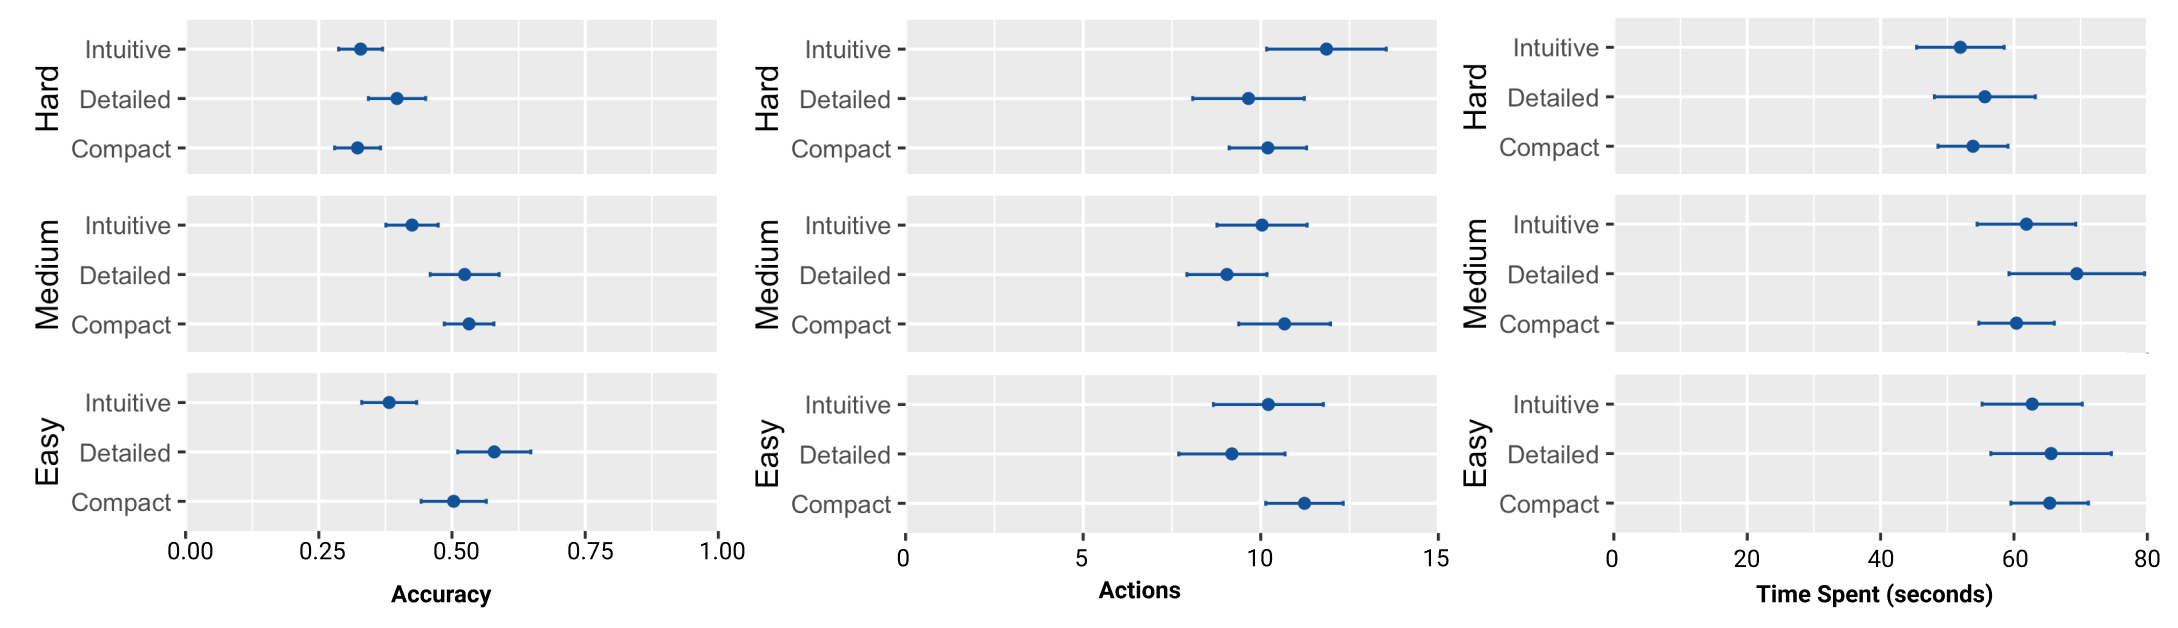
\includegraphics[width=\textwidth]{figures/study1CI.png}
\caption{ Results from \emph{quality of life} study regarding \emph{accuracy}, \emph{actions} and \emph{time spent} each visualisation is grouped by level of difficulty (\emph{easy}, \emph{medium}, \emph{hard}). }\label{study1CI}
\end{figure*} 

\subsection{Results} % (fold)
\label{sec:evaluation}
% =============================================================================

We used an ANOVA to find significance between groups. Independent samples t-test was used to calculate the means with  95\% confidence intervals, results are shown in Figure \ref{study1CI}. For each participant we calculated their \emph{accuracy}, \emph{actions} and \emph{time spent}. We show the results separately for each level of difficulty, \emph{easy}, \emph{medium} and \emph{hard} in Table \ref{tab:results1}. Lastly, we report the results from the 5-Likert scale questionnaire regarding \emph{usability} and \emph{uncertainty} aspects in the visualisations.

\def\arraystretch{1.5}
\begin{table}[t]
  \centering
  \caption{Results from quality of life study. We present with encoded significance, the mean values of each evaluated aspect from participant's responses, grouped by level of difficulty. The values with 95\% confidence intervals are reported in the text.}
    \begin{tabular}{l l l l l }
    \textbf{Aspect} & \textbf{Insight} & \textbf{Intuitive} & \textbf{Detailed} & \textbf{Compact} \\ 
    \hline
    \multirow{3}{*}{Accuracy} & Easy   & 38\% & \textbf{57\%} *** & 50\% *\\
    & Medium & 42\% & 52\% * & \textbf{53\%} ** \\
    & Hard   & 32\% & \textbf{39\%} & 32\% \\
    \hline
    \multirow{3}{*}{Actions} & Easy   & 10.21 & \textbf{9.18} & 11.23 \\
    & Medium & 10.03 & \textbf{9.04} & 10.66 \\
    & Hard   & 11.85 & \textbf{9.65} & 10.19 \\
    \hline
    \multirow{3}{*}{Time} & Easy   & \textbf{62.73s} & 65.57s & 65.36s \\
    & Medium & 61.87s & 69.42s & \textbf{60.38s} \\
    & Hard   & \textbf{51.96s} & 55.63s & 53.86s \\
    \hline
    \multicolumn{2}{l}{Visual appeal   } & \textbf{4} *    & 3 & \textbf{4}\\
    \multicolumn{2}{l}{Ease of use     } & \textbf{3.5}    & 3 & 3         \\
    \multicolumn{2}{l}{Suitability     } & 3   & \textbf{4} * & \textbf{4} \\
    \multicolumn{2}{l}{Liked it        } & 3   & \textbf{4} & 3            \\
    \multicolumn{2}{l}{Tasks were easy } & 2.5 & \textbf{4} * & \textbf{3} \\
    \multicolumn{2}{l}{Trust           } & 3   & 3 & 3                     \\
	\multicolumn{2}{l}{Confidence      } & 3   & 3 & 3                     \\
	\multicolumn{2}{l}{Credibility     } & 3   & 3 & \textbf{4} *          \\
	%\multicolumn{2}{l}{Comprehensible } & 3   & 3 & \textbf{4} *          \\
	\multicolumn{2}{l}{Understanding   } & 3   & 3 & \textbf{4} *          \\
	\multicolumn{2}{l}{Accuracy representation} & 3   & \textbf{4} & \textbf{4}   \\
    \hline
    \multicolumn{5}{c}{
    \footnotesize{
    \makecell{* significant at $p < .05$; ** significant at $p < .01$; \\ *** significant at $p < .001$. The best-scoring values are \textbf{bold}}}
    } \\
    \end{tabular}%
  \label{tab:results1}%
\end{table}%


%\begin{figure}
%\centering
%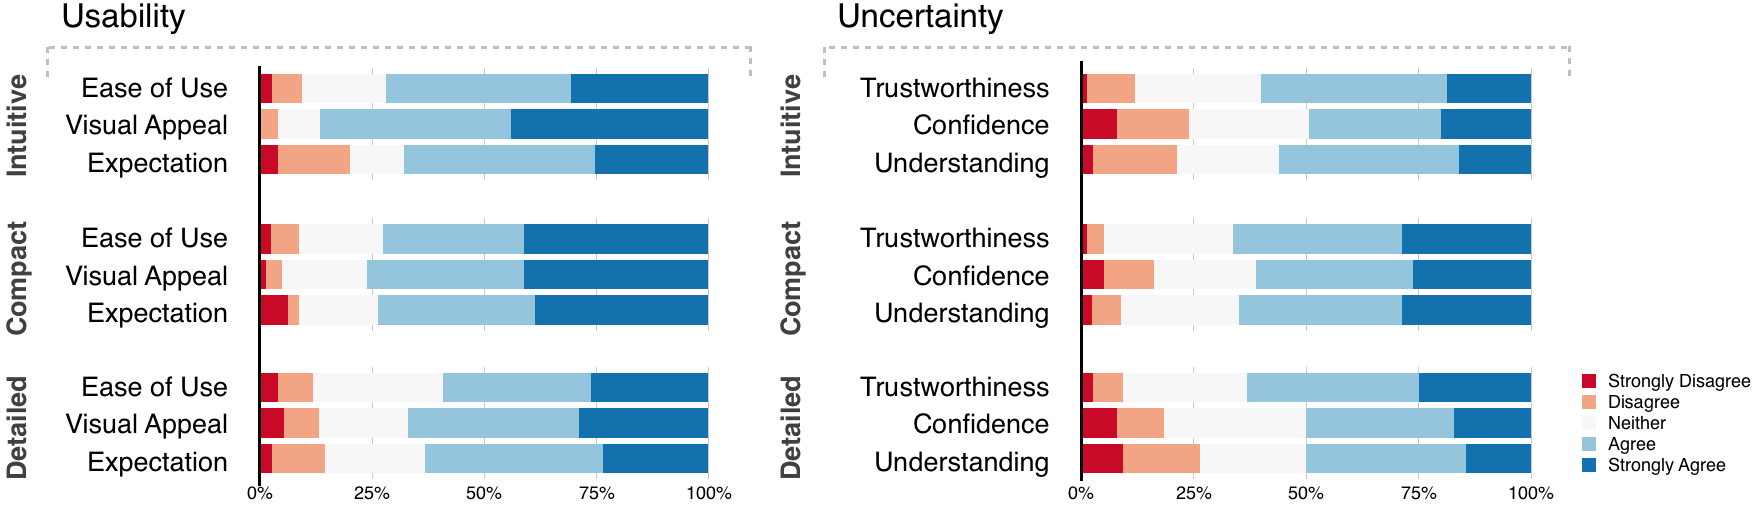
\includegraphics[width=\columnwidth]{figures/study1_qf.png}
%\caption{
%\textbf{Left:} 
%Intuitive visualisation, showing the historical data and forecast using a line chart.
%\textbf{Right:} 
%Detailed visualisation, showing the fitted regression line of the model, together with %observations.}
%\label{study1_qf}
%\end{figure} 

% ////////////// EASY

% Anova 
% easy.accuracy   df=2/209 f=10.178 p=6.055e-05 ***
% medium.accuracy df=2/208 f=5.0692 p=0.007087  **

% Levenes
% medium.speed    2/208 f=4.5    0.01221 *
% medium.accuracy 2/208 f=4.4113 0.0133  *
% easy.accuracy   2/209 f=0.5657 0.5688

% Tukey HSD
% easy.accuracy
% map-chart 0.0000419
% map-dots  0.0119139

% medium.accuracy
% map-chart  0.0302220
% map-dots   0.0107560

\textbf{Easy: Accuracy}. An ANOVA showed an effect on accuracy $(F_{2, 209}=10.178, p < .001)$, A post-hoc Tukey test showed that \emph{intuitive} and \emph{detailed} visualisations differed significantly at $(p < .001)$ and \emph{intuitive} and \emph{compact} visualisations differed significantly at $(p = .03)$. Users tended to be significantly more accurate in the \emph{detailed} visualisation $(mean = 57/100, 95\% CI: [51, 64])$ and \emph{compact} visualisation  $(mean = 50/100, 95\% CI: [44, 56])$ rather than the \emph{intuitive} visualisation $(mean = 38/100, 95\% CI: [33, 43])$. % Ok

\textbf{Easy: Actions}. No significant differences $(F_{2, 209}= 2.21, n.s)$. Interactions tended to be lowest in the \emph{detailed} visualisation $(mean =  9.18, 95\% CI:[7.69, 10.68])$, rather tan \emph{compact} $(mean = 11.23, 95\% CI:[10.14, 12.32])$ or \emph{intuitive}  $(mean = 10.21, 95\% CI:[8.66, 11.76])$  visualisations.

\textbf{Easy: Time spent}. No significant differences were found $(F_{2, 209}= .18, n.s)$. In general, users were faster with \emph{Intuitive} visualisation $(mean = 62.73s, 95\% CI:[55.22, 70.24])$ rather than compact $(mean = 65.36s, 95\% CI:[59.55, 71.17])$ or detailed $(mean = 65.57s, 95\% CI:[56.53, 74.60])$ visualisation.

% ////////////// MEDIUM

\textbf{Medium: Accuracy}. An ANOVA showed an effect on accuracy $(F_{2, 209}=5.06, p = .007)$. A post-hoc Tukey test showed that \emph{intuitive} and \emph{detailed} visualisations differed significantly at $(p = .03)$ and \emph{intuitive} and \emph{compact} visualisations differed significantly at $(p = .01)$. Users tended to be significantly more accurate with the \emph{compact} $(mean = 53/100, 95\% CI:[48, 57])$ visualisation rather than the \emph{intuitive} $(mean = 42/100, 95\% CI:[37, 47])$ visualisation. The \emph{detailed} (mean = 52/100, 95\% CI:[45, 58]) visualisation showed no significant differences between the groups.
 
\textbf{Medium: Actions}. No significant differences $(F_{2, 209}= 1.67, n.s)$, but users tended to require the least interactions using the \emph{detailed} $(mean =  9.04, 95\% CI:[7.91, 10.17])$ visualisation rather than the \emph{intuitive} $(mean = 10.03, 95\% CI:[8.76, 11.30])$ or compact $(mean = 10.66, 95\% CI:[9.37, 11.96])$ visualisations.

\textbf{Medium: Time spent}. No significant differences $(F_{2, 209}= 1.51, n.s)$. Users tended to be faster with the \emph{compact} $(mean = 60.38s, 95\% CI:[54.72, 66.04])$ visualisation. Rather than \emph{intuitive} $(mean = 61.87s, 95\% CI:[54.47, 69.26])$ or \emph{detailed} $(mean = 69.42s, 95\% CI:[59.25, 79.59])$ visualisations.
   
% ////////////// HARD

\textbf{Hard: Accuracy}. No significant differences  $(F_{2, 209}= 3.03, n.s)$. Users tended to be more accurate with \emph{detailed} $(mean = 39/100, 95\% CI:[34, 45])$ visualisation. Rather than \emph{intuitive} $(mean = 32/100, 95\% CI:[28, 36])$ or \emph{compact} $(mean = 32/100, 95\% CI:[27, 36])$ visualisations. 

\textbf{Hard: Actions}. No significant differences $(F_{2, 209}= 2.41, n.s)$. Users tended to be most efficient using the \emph{detailed} $(mean =  9.64, 95\% CI:[8.08,  11.22])$ visualisation, rather than \emph{intuitive} $(mean = 11.85, 95\% CI:[10.16, 13.53])$ or \emph{compact} $(mean = 10.19, 95\% CI:[9.10,  11.28])$ visualisations.

\textbf{Hard: Time spent}. No significant differences $(F_{2, 209}= .31, n.s)$. Users tended to use the least of the time in the \emph{intuitive} $(mean = 51s, 95\% CI:[45s, 58s])$ condition. Rather than \emph{compact} $(mean = 53s, 95\% CI:[48s, 59s])$ or \emph{detailed} $(mean = 55s, 95\% CI:[48s, 63s])$ visualisations.

For the results from the posterior questions related to \emph{usability} and \emph{uncertainty}. We used a Kruskal Wallis U non-parametric test to find a significance in the responses. Mann-Whitney tests were used as a follow-up to the findings. A Bonferroni correction was applied and so all effects are reported at .016 level of significance.
%Results are depicted in Figure \ref{likert-s1-usability}.

%\begin{figure}
%\centering
%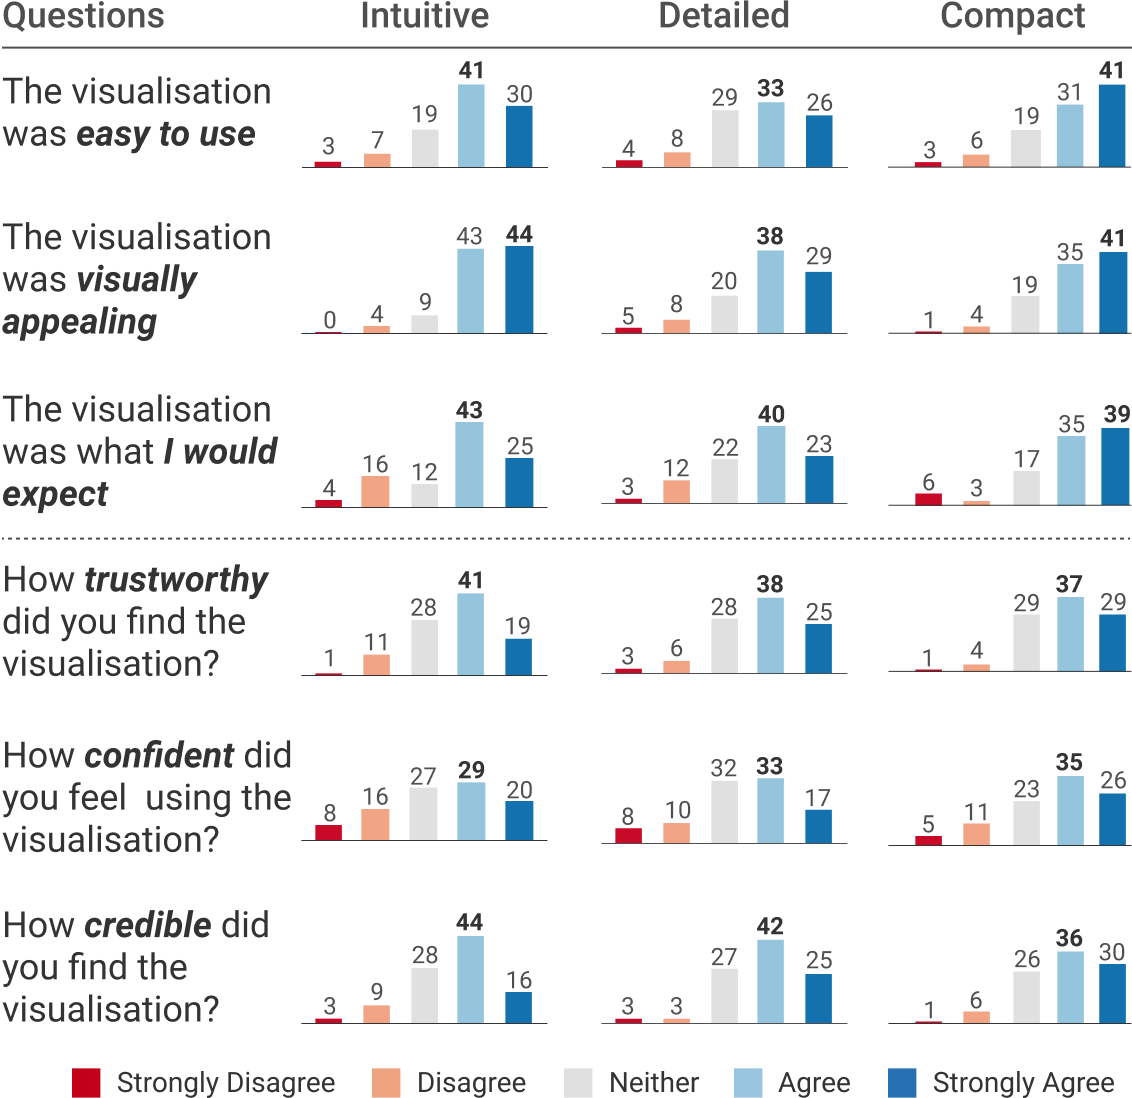
\includegraphics[width=0.5\textwidth]{figures/likert-s1-usability.png}
%\caption{Percent of Likert-scale responses in the first study. \textbf{Top}: Attitudes towards \emph{usability}. \textbf{Bottom}: Attitudes towards \emph{uncertainty}, highest scores are highlighted in \textbf{bold}.}
%\label{likert-s1-usability}
%\end{figure}

%%% Usability

\textbf{Usability: Visual Appeal.} People's attitudes towards visual appeal were significantly affected by the visualisation given to them $(H(2) = 7.77, p  = .02)$. It appeared that visual appeal was significantly higher for \emph{intuitive}  $(Mdn = 4)$ rather than \emph{detailed} visualisation $(Mdn = 3),  W = 536, p = .035$. However, no significant differences were found towards \emph{compact} visualisation $(Mdn = 4)$.

\textbf{Usability: Ease of use.} No significant differences were found. The median for \emph{compact}, \emph{intuitive} and \emph{detailed} visualisations was 4. The median indicates an equal rank for all visualisations. However, best scores show a ranking from high to low in the order of $compact > intuitive > detailed$.

%\textbf{Usability: Expectation.} No significant differences were found. The median for \emph{compact}, \emph{intuitive} and \emph{detailed} visualisations was 4. The median indicates an equal rank for all visualisations. Best scores indicate a ranking from high to low in the order of $intuitive > compact > detailed$.

\textbf{Usability: Suitability.} People thoughts about visualisation suitability differed significantly $(H(2) = 7.49, p = .02)$.  \emph{Detailed} visualisation $(Mdn = 4)$ appeared to be significantly more suitable rather than \emph{intuitive} $(Mdn = 3, w = 263, p = .04)$ and \emph{compact} $(Mdn = 4, w = 543, p = .04)$ visualisations.

\textbf{Usability: Liked it.} No signficant differences were found. Participants tended to show preference for the detailed visualisation $(Mdn = 4)$, rather than \emph{compact} or \emph{intuitive} visualisations $(Mdn = 3)$. 

\textbf{Usability: Tasks were easy.} People thoughts about the difficulty of tasks differed significantly depending on the visualisation $(H(2) = 7.52, p < .02)$. Participants that used the \emph{detailed} visualisation $(Mdn = 4)$ though the tasks were easy to solve, rather than \emph{compact} $(Mdn = 3)$ or intuitive $(Mdn = 2.5)$.


%%% Uncertainty..

\textbf{Uncertainty: Trust.} No significant differences were found. The median for \emph{compact}, \emph{intuitive} and \emph{detailed} visualisations was 4. The median indicates an equal rank for all visualisations. Best scores indicate a ranking from high to low in the order of $intuitive > compact > detailed$.


\textbf{Uncertainty: Confidence.} People's confidence in their responses were significantly affected by the visualisation given to them $(H(2) = 6.45, p = 0.03).$  However, post-hoc analysis showed no significant differences to report. The median in \emph{compact}, \emph{intuitive} and \emph{detailed} visualisations was 3. 

\textbf{Uncertainty: Credibility.} We found a significant difference in participants opinions towards credibility  $(H(2) = 6.85, p = 0.03).$. Indicating that \emph{compact} $(Mdn = 4)$ visualisation appeared to be more credible than \emph{detailed} $(Mdn=3, w=645, p=0.03)$,  visualisation. No significant differences were found against \emph{intuitive} $(Mdn=3)$.

\textbf{Uncertainty: Understanding} We found a significant effect in the visualisations regarding uncertainty understanding, indicating that the \emph{compact} $(Mdn = 4)$ visualisation was greater than \emph{intuitive} visualisation  $(Mdn = 3, p < 0.05)$. No significant differences were found for \emph{detailed} visualisation. $(Mdn = 4)$.

\textbf{Uncertainty: Accuracy Representation.} No significant differences were found. However people tended to prefer the accuracy representation in \emph{detailed} $(Mdn=4)$ and \emph{compact} $(Mdn=4)$ visualisations rather than the \emph{intuitive} $(Mdn=3)$.

\subsection{Summary}

\textbf{Intuitive} visualisation, the use of Chernoff-faces as the  had a significant impact in the evaluation. Results indicated that the selection of a suitable visualisation is important and makes a big difference in overall accuracy and number of interactions. Even though their accuracy score was not the best, participants praised the visualisation by its visual appeal $(Mdn = 4)$. However, they indicated that the tasks seemed more difficult using this visualisation $(Mdn = 2.5)$. Uncertainty measures are not clear, participants tended to show a neutral opinion $(Mdn = 3)$, so further investigation is required in this regard.

\textbf{Detailed} visualisation, in general, participants were more accurate. However, they showed neutral attitudes towards uncertainty factors like trust,  confidence, credibility and understanding $(Mdn = 4)$. However they thought that the visualisation was suitable and the task seemed easy to solve $(Mdn = 4)$.

\textbf{Compact} visualisation, participants tended to be less accurate for hard-level tasks. They rated the visualisation positively for credibility, understanding and accuracy representation $(Mdn = 4)$. However they were more conservative in other factors such as trust, confidence and ease of use $(Mdn = 4)$.


%\def\arraystretch{1.5}
%\begin{table}[b!]
 % \centering
  %\caption{5-Likert scale results from quality of life study. We present with encoded significance, the median values of each evaluated aspect from participant's responses, grouped by visualisation.}
   % \begin{tabular}{p{0.35\linewidth} l l l }
    %\textbf{Question} & \textbf{Intuitive} & \textbf{Detailed} & \textbf{Compact} \\ 
    %\hline
    %The visualisation was \textbf{easy to use}. & 4 & 4 & 4         \\
    %The visualisation was visually \textbf{appealing}. & 4 & 4 & 4  \\
    %The visualisation was what I would \textbf{expect}. & 4 & 4 & 4 \\
    %How \textbf{trustworthy} did you find the visualisation? & 4 & 4 & 4 \\
    %How \textbf{confident} did you feel answering questions using the visualisation? & 4 & 3 & 3.5 \\
    %%How \textbf{credible} did you find the visualisation? & 4 & 4 & 4 \\
    %%\hline
    %\multicolumn{4}{c}{
    %\footnotesize{
    %\makecell{* significant at $p<0.5$; ** significant at $p<0.01$; \\ *** significant at $p<0.001$. The best-scoring values are \textbf{bold}}}} \\
    %\end{tabular}%
  %\label{tab:qualitative1}%
%\end{table}%


% Charts:
% ALL:
% - time spent,
% - comparatively high accuracy
% - high efficiency


% Dots:
% low 
% high eff
% time spent

% med
% spent more time.
% high acc


% Map:
% Low
% - high acc

% Mid:
% - low all

% Hard:
% - Time spnt

\section{Second study: financial decisions}

To generalise the findings of the first user study, we replicated the design motivations and evaluation in a second, and different, context. In this second user study, we collected financial data and designed and implemented intuitive, compact and detailed model representations on top of this data to support decision-making for non-expert users.  

\subsection{Design Motivation}

A typical scenario for decision-making is the investment in stock prices. Such a task is subject of heavy uncertainty due to many variables that are involved. We used data related to stock prices to compare the utility of different model representations for decision-making process for non-experts in this second user study.

\textbf{What and When: Intuitive Representation \emph{(time series)}}. Investing capital in stocks requires to see the behavior of the company stock price in the past. Typically, stock prices fluctuate a lot over time, depending on different factors, such as worldwide news, oil price, and world economy. For the intuitive representation we decided to ask to a financial expert about typical time series visualisation. Based on the expert feedback we came down to a time series visualisation showing the last year historic fluctuation of the stock value and the next year forecast. The time-series visualisation is suited for answering simple questions concerning aspects of what and when.

\textbf{Why: Detailed Representation \emph{(scatter plot)}}. As in the previous study a detailed visualisation of the prediction model allows users to investigate why and how a prediction is made. By inspecting the variables in the model, users can identify possible sources of uncertainty. Differences between the distributions of observations can be depicted and users can see how data is correlated. As the approach requires a certain degree in graph literacy, it is important to investigate when and how such a representation is appropriate to support decision-making for non-expert users.

\textbf{How: Compact Representation \emph{(dot plot)}}. As a third representation we included the dot plot visualisation, which was used previously in the first study. We were curious on how compact visualisations perform in different scenarios within different levels of insight. The visualisation focuses on showing the probability of an event to happen. The representation is less detailed as the scatter plot representation, as it does not represent the observations and model. However, it does show a clear representation of the chance of future events to happen. 

\textbf{Uncertainty}. To consider uncertainty in the visualisation, it is important to correctly interpret a model's prediction. As in our previous study, we used different levels of opacity to represent the value of accuracy among the visualisations. We showed the prediction intervals divided by quantiles. Then, we used opacity (from light grey to dark grey) to represent accuracy (from unlikely to likely) across all the three visualisations.

\subsection{Application design}
We created a set of visualisations to represent the predicted stock price for different companies. A different visualisation was used for each of the three study applications resulting in three identical applications, one with a set of six intuitive visualisations, a second with a set of six compact visualisations and a third with a set of six detailed visualisations. The application can be separated and described in the following modules: 

\subsection{Data}
We used the Quandl API\footnote{https://www.quandl.com/docs/api} to get the current and historical records of stocks from Dow Jones companies. We also used the Twitter streaming API to track financial topics such as worldwide news, costumer confidence, and economic growth that might have an impact on the stock market \citep{Bollen2011}. This data was analysed by a financial expert who identified different variables for training the model (consumer trust, worldwide news, economic growth, and Dow Jones index), the time period most relevant to consider (January 2015 to March 2016), and how this data should be displayed. We selected six popular companies from the Dow Jones share that had a similar behavior in their stock prices: Disney (NYSE: DIS), Home Depot (NYSE: HD), Apple (NASDAQ: AAPL), Chevron (NYSE: CVX), IBM (NYSE: IBM), and McDonalds (NYSE: MCD). 

\subsection{Model}
The prediction model was defined by a regression model. We created a model that included consumer trust, worldwide news, economic growth, and the Dow Jones index as the prediction variables. The algorithm returned a prediction of the stock price for the next year.

\subsection{Interaction}
Each application was divided in three main sections: settings, visualisation and questions. The settings section showed the four prediction variables that were integrated into the model (consumer trust,  worldwide news, economic growth, and Dow Jones index). The variables were shown as checkboxes with sliders, as presented in Figure \ref{whole_app2}. Selecting the checkbox determines whether the variable is to be considered into the prediction. Each slider enables the user to set the level of importance of this variable in the model. When the user selects different variables or changes their importance with sliders, the visualisation is updated in real-time. Next, a questions section shows a set of easy-to-hard questions reviewed by the financial expert. The users had to interact with a combination of variable settings in order to respond to all the questions.

\begin{figure*}
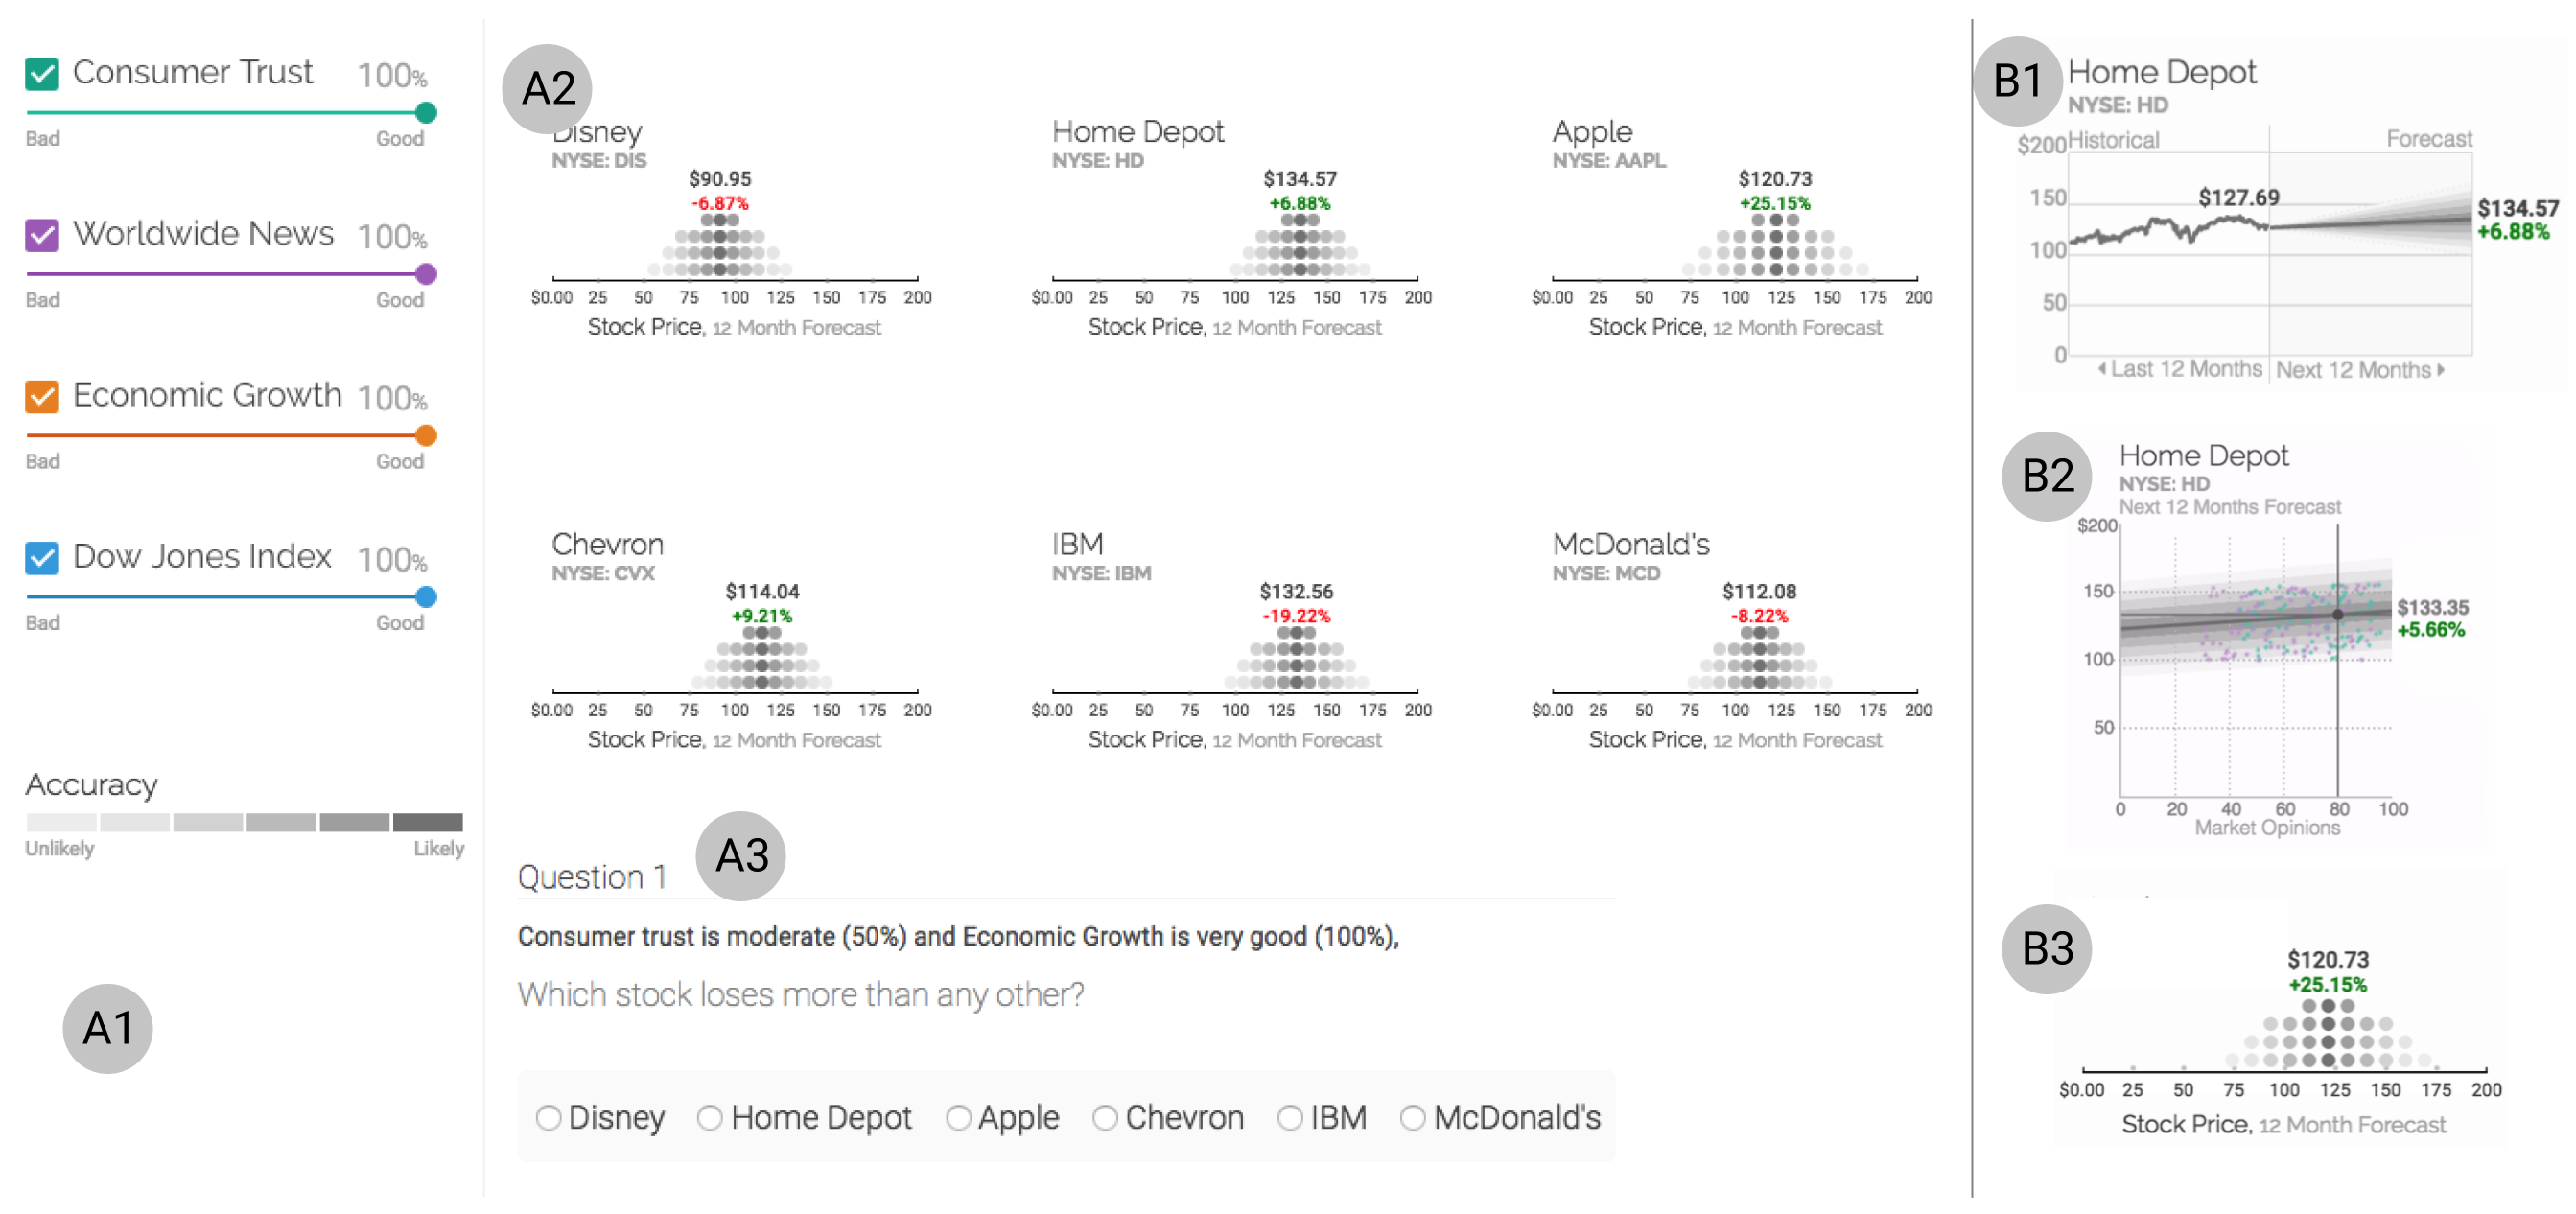
\includegraphics[width=\textwidth]{figures/whole_app2.png}
\caption{\textbf{A) Left:} Screen shot of the main screen in the application. \textbf{A1.} \textbf{Settings section}, where users selected the values for the prediction variables. \textbf{A2.} \textbf{Visualisations section}, where the predictions were shown using different levels of opacity to represent accuracy. \textbf{A3} \textbf{Questions Section}, users had to interact with the settings and see the results in the visualisations to select the correct answer. \textbf{B) Right:} The three different visualisations used to represent the predictions. \textbf{B1.} \textbf{Intuitive} visualisation. \textbf{B2.} \textbf{Detailed} visualisation. \textbf{B3.} \textbf{Compact} visualisation.}\label{whole_app2}
\end{figure*} 

\subsection{Visualisation}
The intuitive, compact and detailed visualisations as presented in Figure \ref{whole_app2} were separated in three different applications. Each of the visualisations represented stock price predictions of the same six companies.

\textbf{Figure \ref{whole_app2}, B1:  Intuitive visualisation (time series)}. In this visualisation the stock prices predictions were shown using time series. We implemented a line chart to show the variation of the stock price divided in two sections: historical and forecast. The historical section depicted the stock prices from the last 12 months as historical data. The forecast section showed the expected predicted value for the next 12 months. We also showed the value of the last stock price for the historical data, the value of the forecasted stock price and the percentage difference between these two values, coloured by red (negative) or green (positive). In addition, we showed the prediction interval for such a prediction. We used an opacity scale that indicated the likelihood for the predicted value from unlikely (light grey) to likely (dark grey). In other words, the opacity scale highlighted the quantiles of the predicted probability distribution and showed the range of accuracy for the value. The visualisation was updated immediately after when the user adjusted the importance of different variables in the settings section.

\textbf{Figure \ref{whole_app2}, B2: Detailed visualisation (scatter plot)}. The visualisation consists of the plot of the regression model together with the observations of each variable. The spread of stock prices of a risk was mapped to the X-axis, the corresponding distribution of the variables describing the economic factors to the Y-axis and then plotted into the coordinate system. The predicted value for the stock price was written in text next to the visualisation at the Y- coordinate of the corresponding point of the regression line.


\textbf{Figure \ref{whole_app2}, B3: Compact visualisation (dot plot)}. The visualisation represents the quantiles in a probability distribution. Previously it has been discussed that a dot visualisation facilitates the communication of probability as countables \citep{Garcia-retamero2016}. We used opacity in the dots to represent the accuracy for the stock price from unlikely (light grey) to likely (dark grey). The most likely predicted stock value was shown above the mean of the probability distribution. The percentage difference was diplayed below. Color was used to depict increase (green) or decrease (red) of the stock price.


\subsection{Study formulation}
The financial expert analysed the data, model and visualisations to create a set of 20 candidate questions. From this set we selected 12 questions for the study. Questions were separated equally into three different categories according to their difficulty (easy, medium and hard). We measured the difficulty of the questions by the number of variables involved and the interactions needed to solve them. We implemented the same questions into the three applications. The order of the questions in each study was randomized.
			
\subsection{Main study}

We recruited 360 users on Amazon Mechanical Turk (AMT), 120 per application. To  participate in the study users were required to have a minimum HIT approval rate of 95\%. We included verification questions to detect if users were cheating. As in the previous study, these were simple questions that used similar controls as the normal questions (e.g. \q{What is 5 + 3?}). If any of these \q{gold} questions were wrong the participation of the user was not considered in the final results. In addition, we offered a short tutorial at the beginning of the evaluation, explaining the variables, model and visualisations. We added five training questions to help users familiarise themselves with the application. 

Each user could only participate once and received a minimum payment of \$0.50. Like in the first study, to motivate users, we offered bonuses: For answering at least 66\% of questions correctly, users received \$2.50, for more than 80\%, they received \$3.50.

The application was presented in a desktop Web browser. The application was designed for a view of 800w x 600h pixels to ensure the compatibility with different screen sizes. The position of all the view components were the same in the three applications.  By default, the values for variables in the settings were turned off and started from zero. 

% The position order for the companies in the main visualisation section from left to right were the following, first row: Disney, Home Depot, Apple, second row: Chevron, IBM, McDonald's. 

After a short tutorial that described all the concepts of the application, users were able to start the evaluation. For all the twelve questions the process was the same. Users were shown a question and then they clicked a start button. After clicking this start button, the settings, controls and visualisations became visible. Only after dragging or clicking on the sliders the submit button to send the answer appeared to ensure that users could not skip answers. The process was repeated for each question (twelve times) during the study. We recorded time, interactions with variables (slider and checkbox) and given answers. Recording started right after users clicked the start button, and ended when they pressed the submit button.

To investigate the effect of the visualisations on perceptions, we asked users to respond six Likert-scale questions on a five point scale (one: strongly disagree, five: strongly agree)  regarding usability (\emph{visual appeal}, \emph{ease of use}, \emph{suitability}, \emph{liked it}, \emph{ease of tasks}) and uncertainty (\emph{trust}, \emph{confidence}, \emph{credibility}, \emph{understanding}, \emph{accuracy representation}).

Users who had failed more than one of the verification questions, had less than three correct answers or did not finish the evaluation were removed from the data, leaving the following group sizes: \textit{Intuitive}: 101 users (38F, 62M, 1PNS; mean age: 32.3, SD: 8.9); \textit{Detailed}: 86 users (57M, 29F; mean age: 34.8, SD: 10.5) \textit{Compact}: 84 users (28F, 54M, 2PNS; mean age: 32.5, SD: 9.47), . The average time of the study for each participant was about 21 minutes. 

\def\arraystretch{1.5}
\begin{table}[t]
  \centering
  \caption{Results from financial decisions study. We present the mean values of each evaluated aspect from participant responses, with encoded significance and grouped by level of difficulty (easy, medium, hard). The values with 95\% confidence intervals are reported in the text.}
    \begin{tabular}{l l l l l }
    \textbf{Aspect} & \textbf{Insight} & \textbf{Intuitive} & \textbf{Detailed} & \textbf{Compact} \\ 
    \hline
    \multirow{3}{*}{Accuracy} & Easy   & 71\% & \textbf{72\%}   & 64\% \\
                              & Medium & \textbf{85\%} *        & \textbf{85\%} * & 75\% \\
                              & Hard   & 75\% & \textbf{79\%} * & 70\% \\
    \hline
    \multirow{3}{*}{Actions} & Easy   & 7.57 & 6.94 & \textbf{6.65} \\
                             & Medium & 7.52 & \textbf{6.42} * & 6.68 \\ 
                             & Hard   & 8.73 & 8.24 & \textbf{7.69} \\
    \hline
    \multirow{3}{*}{Time} & Easy & 59.74s & 65.57s & \textbf{55.74s} \\
    & Medium & 50.75s & \textbf{46.41s} & 47.85s \\
    & Hard   & 54.02s & 52.25s & \textbf{50.54s} \\
    \hline
    \multicolumn{2}{l}{Visual appeal    } & \textbf{5} & 4 & 4 \\    
    \multicolumn{2}{l}{Ease of use      } & \textbf{5} * & 5 & 4 \\
    %\multicolumn{2}{l}{Expectation     } & \textbf{4} & 4 & 4 \\
    \multicolumn{2}{l}{Suitability      } & \textbf{5} *** & \textbf{5} ** & 4 \\
    \multicolumn{2}{l}{Liked it         } & \textbf{5} & 4 & \textbf{5} \\
    \multicolumn{2}{l}{Tasks were easy  } & \textbf{5} *** & 4 * & 3 \\
    \multicolumn{2}{l}{Trust            } & \textbf{4} **  & 4 & 3 \\
    \multicolumn{2}{l}{Confidence       } & \textbf{5} ** & 4.5 ** & 3 \\
    \multicolumn{2}{l}{Creadibility      } & 4 & 4 & 4   \\
    %\multicolumn{2}{l}{Comprenhensible    } & \textbf{5} *** & 4 * & 3.5 \\
    %\multicolumn{2}{l}{Operation        } & \textbf{5} *** & \textbf{5} ** & 3.5 \\
    \multicolumn{2}{l}{Understanding    } & \textbf{5} **  & \textbf{5} & 4 \\
    \multicolumn{2}{l}{Accuracy representation} & \textbf{5} & 4 & 4   \\
    %\multicolumn{2}{l}{Engaging          } & \textbf{5} & \textbf{5} & 4   \\
    %\multicolumn{2}{l}{Uncert. Importance} & \textbf{5} *** & 4 & 4   \\
    %\multicolumn{2}{l}{Opacity           } & \textbf{4} & 4 & 4 \\
    \hline
    \multicolumn{5}{c}{
    \footnotesize{
    \makecell{* significant at $p < .05$; ** significant at $p < .01$; \\ *** significant at $p < .001$. The best-scoring values are represented in \textbf{bold}.}}
    } \\
    \end{tabular}%
  \label{tab:results2}%
\end{table}%

\begin{figure*}
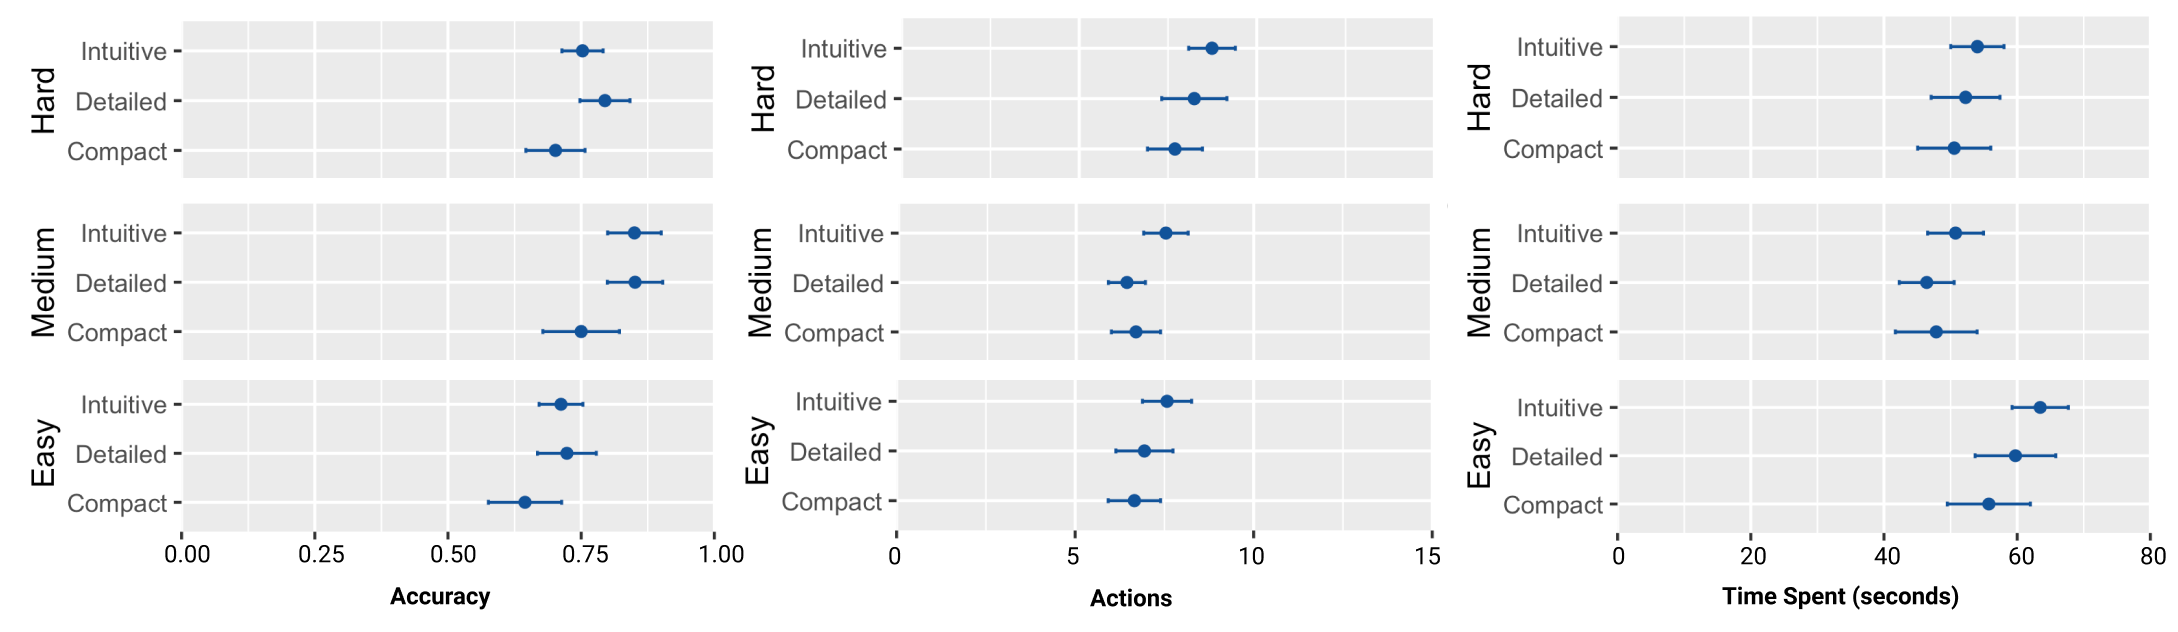
\includegraphics[width=\textwidth]{figures/study2CI.png}
\caption{Evaluation results from the second study, financial decisions. \textbf{Left:} \textit{(accuracy)}, participants where more accurate solving medium difficulty questions. \textbf{Middle:} \textit{(actions)}, Users tended to require less actions in the second study \textbf{Right:} \textit{(time spent)}, Users tended to be faster with their decisions in the second study. }\label{study2CI}
\end{figure*} 

\subsection{Results}
We used an ANOVA to find significance between the groups. Results are shown in in Table \ref{tab:results2}. Independent samples t-test was used to calculate the 95\% confidence intervals, see Figure \ref{study2CI}. We also show the results of the 5-Likert scale questions on participant attitudes towards \emph{usability} and \emph{uncertainty}. 
 
% Easy accuracy                           *** 0.0003798
% leveneTest(medium.accuracy, medium.viz) **  0.008926
% leveneTest(hard.accuracy  , hard.viz)   *   0.01191

\textbf{Easy: Accuracy}. No significant differences $(F_{2, 263} = 2.28, n.s)$. Users tended to be more accurate using the \emph{detailed} visualisation $(mean=72/100, 95\% CI:[66,77])$ and the \emph{intuitive} visualisation $(mean=71/100, 95\% CI:[67,75])$ rather than \emph{compact} visualisation $(mean=64/100, 95\% CI:[57,71])$.
 
\textbf{Easy:  Actions}. No significant differences $(F_{2, 263} = 1.65, n.s)$. Interactions tended to be lowest in the \emph{compact} visualisation $(mean = 7.6, 95\% CI: [6.9, 8.4])$ rather than \emph{detailed} $(mean = 8.24, 95\% CI: [7.3, 9.1])$ or \emph{intuitive} $(mean = 7.6, 95\% CI: [6.9, 8. ])$  visualisations.

\textbf{Easy:  Time Spent}. No significant differences $(F_{2, 263} = 2.28, n.s)$. Users tended to complete each task faster with the \emph{compact} visualisation $(mean = 55s, 95\% CI: [49, 61])$ rather than \emph{detailed} $(mean = 59s, 95\% CI: [55, 65])$  or \emph{intuitive} $(mean = 63s, 95\% CI: [59, 67])$  visualisations.

\textbf{Medium:  Accuracy}. An ANOVA showed an effect of visualisation on accuracy $(F_{2, 264} = 3.81, p = .023)$. Tukey HSD post hoc analysis revealed significant differences between \emph{compact} and \emph{detailed} visualisations $(p < 0.047)$, \emph{compact} and \emph{intuitive} visualisations $(p < 0.03)$, no significant differences between \emph{detailed} and \emph{intuitive} visualisations were found $(n.s)$. Accuracy was highest for \emph{detailed} visualisation $(mean = 85/100, 95\% CI: [79, 90])$ and \emph{intuitive} $(mean = 85/100, 95\% CI: [79, 90])$ visualisation rather than \emph{compact} visualisation $(mean = 75, 95\% CI: [67, 82])$.

\textbf{Medium:  Actions}. An ANOVA showed an effect of visualisation on interactions ($F_{2, 264} = 3.56, p = .029)$. A Tukey HSD post hoc analysis revealed significant differences between \emph{intuitive} and \emph{detailed} visualisations $(p < 0.03)$. No other significant differences where found. Users tended to require the least interactions using the \emph{detailed} visualisation $(mean = 6.4, 95\% CI: [5.9, 6.9])$ rather than the \emph{intuitive} $(mean = 7.5, 95\% CI: [6.9, 8.1])$ or \emph{compact} $(mean = 6.6, 95\% CI: [5.9, 7.3])$ visualisations. 

\textbf{Medium:  Time Spent}. No significant differences $(F_{2, 263} = .52, n.s)$. Users tended to be faster with the \emph{detailed} visualisation $(mean = 46s, 95\% CI: [42, 50])$, rather than the \emph{compact} $(mean = 47s, 95\% CI[41,53])$ and the \emph{intuitive} $(mean = 50s, 95\% CI[46,54])$ visualisations.

\textbf{Hard:  Accuracy}. An ANOVA showed an effect of visualisation on accuracy ($F_{2, 264} = 3.81, p = .026)$. A Tukey HSD post hoc analysis revealed significant differences between \emph{compact} and \emph{detailed} visualisation $(p<0.019)$.  Users were more accurate using the \emph{detailed} visualisation $(mean = 79/100, 95\% CI: [74, 84])$ rather than the \emph{compact} $(mean = 70/100, 95\% CI: [64, 75])$ or \emph{intuitive} $(mean = 75/100, 95\% CI: [71, 79])$ visualisations.

\textbf{Hard:  Time Spent}. No significant differences $(F_{2, 263} = .52, n.s)$. Users tended to be faster with the \emph{compact} visualisation
$(mean = 50s, 95\% CI: [45, 56])$ rather than \emph{intuitive} $(mean = 54s, 95\% CI: [50, 58])$ or  \emph{detailed} $(mean = 52s, 95\% CI: [47, 57])$ visualisations.

\textbf{Hard:  Actions}. No significant differences $(F_{2, 263} = 1.82, n.s)$. Users tended to be more efficient using the \emph{compact} visualisation $(mean = 7.67, 95\% CI: [6.92, 8.46])$ rather than \emph{intuitive} $(mean = 8.7, 95\% CI: [8.0, 9.3])$ or \emph{detailed} $(mean = 8.2, 95\% CI: [7.3, 9.1])$ visualisations.

For participant's posterior feedback we used a Kruskal Wallis U non-parametric test to find a significance in the responses related to \emph{usability} and \emph{uncertainty}. Mann-Whitney tests were used as a follow-up in the findings. A Bonferroni correction was applied and so all effects are reported at .016 level of significance.
%Results are depicted in Figure \ref{likert-s2-usability}.

%\begin{figure}
%\centering
%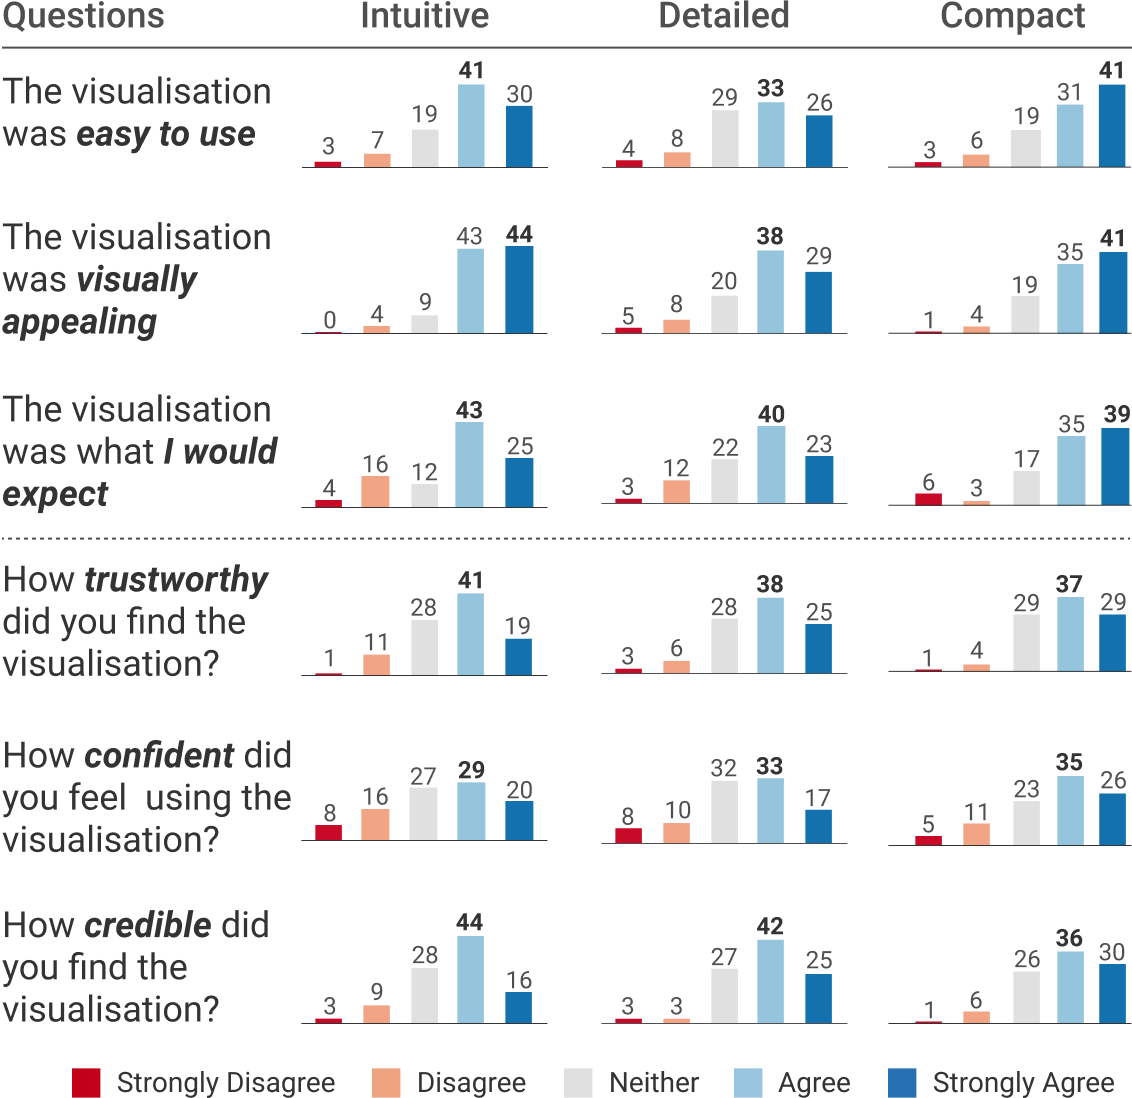
\includegraphics[width=0.5\textwidth]{figures/likert-s1-usability.png}
%\caption{Results of the Likert-scale questions for the second study on attitudes towards usability and uncertainty in the visualisations. The best scores are highlighted in \textbf{bold}.}
%\label{likert-s2-usability}
%\end{figure}

% Usability

\textbf{Usability: Visual Appeal.}  No significant differences were found. The median for \emph{compact}, \emph{intuitive} and \emph{detailed} visualisations was 4. The median indicates an equal rank for all visualisations.

\textbf{Usability: Ease of use.} We found significant differences in people's thoughts towards ease of use $(H(2) = 7.84, p = .019)$. The \emph{intuitive} visualisation $(Mdn = 5)$ appeared to be significantly better than \emph{compact} $(Mdn = 4)$ $w = 86.5, p = 0.036$. There were  significant differences in comparison to the \emph{detailed} $(Mdn = 5)$ visualisation. 

\textbf{Usability: Suitability.} Significant differences were found $(H(2) = 19.36, p < .001)$. A post-hoc analysis showed that participants thought that the \emph{detailed} $(Mdn = 5, w = 266.5, p < 0.001)$ and \emph{intuitive} $(Mdn = 5, w = 44.5, p < 0.001$) visualisations were more suitable compared to the compact $(Mdn = 3.5)$ visualisation.

\textbf{Usability: Liked It.} We discovered a significant difference between participant's responses towards likeness $(H(2) = 7.29, p = .02)$. Follow-up studies showed no significant differences. However, the medians indicate that people liked the \emph{compact} and \emph{intuitive} $(Mdn = 5)$ visualisations more than the \emph{detailed} $(Mdn = 4)$ visualisation.

%\textbf{Usability: Engagement.} Kruskal-Wallis test indicated a significant difference between participant's responses $(H(2) = 6.8, p = .033)$. However after running follow-up studies no significant differences were found. The medians indicate that detailed $(Mdn=5)$ and intuitive $(Mdn=5)$ visualisations where more engaging than compact $(Mdn=4)$ visualisations.

%\textbf{Usability: Operation.} Significant differences were found $(H(2) = 18.63, p < .001)$. Post-hoc analysis showed that participants tended to prefer the operability of detailed $(Mdn = 5), w = 253, p < 0.001$ and intuitive $(Mdn = 5), w = 60, p < 0.001$ rather than compact $(Mdn = 3.5)$ visualisation.


\textbf{Usability: Tasks were easy.} Significant differences were found $(H(2) = 16.23, p < .001)$. A post-hoc analysis showed that participants thought that the \emph{intuitive}  $(Mdn = 5, w = 43.5, p < 0.001)$ and \emph{detailed} $(Mdn = 4, w = 247.5, p = 0.005)$ visualisations were significantly more suitable for solving the tasks than the \emph{compact} $(Mdn = 3)$ visualisation.

%%% Uncertainty..

%\textbf{Usability: Opacity Depiction.} Significant differences were found $(H(2) = 7.77, p < .02)$. Post-hoc analysis showed that participants thought that intuitive  $(Mdn = 5), w = 43.5, p < 0.001$ and detailed $(Mdn = 4), w = 247.5, p = 0.005$ were significantly more suitable vis

\textbf{Uncertainty: Trust.} Significant differences were regarding trust in the visualisations $(H(2) = 13.09, p = .001)$. Participants tended to trust the \emph{intuitive} $(Mdn = 4, W = 58.5, p < .001)$ visualisation more than the \emph{compact} $(Mdn = 3)$ visualisation. No significant differences were found for the \emph{detailed} $(Mdn = 4)$ visualisation.

\textbf{Uncertainty: Confidence.} Significant differences were found $(H(2) = 17.63, p < .001)$. A post-hoc analysis showed that participants tended to be more confident with their decisions using the \emph{intuitive} $(Mdn = 5, w = 41.5, p < 0.001)$ or \emph{detailed} $(Mdn = 4.5, w = 253, p < 0.001)$ visualisations  than the \emph{compact} visualisation $(Mdn = 3)$.

\textbf{Uncertainty: Credibility.} No significant differences were found. Participant's thoughts towards credibility of visualisation were in general positive $(Mdn = 4)$.

%\textbf{Uncertainty: Comprehensible.} Significant differences were found $(H(2) = 15.26, p < .001)$. Post-hoc analysis showed that participants thought that intuitive  $(Mdn = 5), w = 52.5, p < 0.001$ and detailed $(Mdn = 4), w = 245.5, p = 0.005$ were significantly more comprehensible than compact $(Mdn = 3.5)$ visualisation.

\textbf{Uncertainty: Understanding.}  Kruskal Wallis test indicated significant differences in people's thoughts towards visualisation understanding $(H(2) = 12.03, p = .002)$. We discovered that the \emph{intuitive} $(Mdn = 5,  w=57.5, p < 0.001)$ visualisation   was significantly better to understand than the \emph{compact} $(Mdn = 4)$ visualisation. No significant differences were found for the \emph{detailed} $(Mdn = 5)$ visualisation.

\textbf{Uncertainty: Accuracy representation.} Significant differences were found $(H(2) = 15.05, p < .001)$. Participants thought that showing accuracy was more important in the \emph{intuitive} $(Mdn = 5, w = 50, p < 0.001)$ visualisation rather than the \emph{compact} $(Mdn = 4)$ visualisation. No significant differences where found towards the  \emph{detailed} visualisation.

%%%
\subsection{Summary}

Overall, participants that used the \emph{intuitive} visualisation tended to be more accurate for medium and easy-level tasks than for hard-level tasks. Participants that were accurate reported that the visualisation was easy to use $(Mdn = 5)$, and they felt confident when they used it $(Mdn = 5)$.

Participants that used the \emph{detailed} visualisation were in general the most accurate. In general participants needed less actions and spent less time to solve tasks than with the intuitive visualisation, but more actions and time than with the compact visualisation. Participants reported that the visualisation was suitable for solving the tasks (Mdn = 5) and they felt confident about it $(Mdn = 4)$. They also had a positive attitude towards understanding $(Mdn = 5)$.

Participants tended to perform the least actions with the \emph{compact} visualisation and needed less time, but they were, in general, the least accurate. Participants rated credibility slightly higher for the compact visualisation than for the other two visualisations. They showed a positive attitude towards liking the visualisation $(Mdn = 5)$ but they were not sure about uncertainty factors like trust and confidence $(Mdn = 3)$. However they rated the visualisation positively towards credibility, accuracy representation and understanding $(Mdn = 4)$.

%and mentioned that it was engaging $(r = 0.25, n = 240, p < 0.001)$ \kv{we don't describe the engagement results now?}. Even though the correlation between understanding and accuracy was positive it was not significant.

\section{User study 1 vs User study 2}

In this section we summarise and discuss the results from the first and the second user studies. To compare participants accuracy, actions and time spent, we estimate the difference in variance for each visualisation. %and level of difficulty of the tasks
This allowed us to tell how many times people performed with one visualisation compared to another in the two studies by looking at the baseline (no effect). In Figure \ref{vizFigures3} we describe the results from the two studies with 95\% confidence intervals depicted in a forest plot.

We describe the comparison of the visualisations by accuracy, actions and time spent. Then, we discuss the overall results and provide recommendations based on the uncertainty and usability findings. 

\begin{figure*}[t]
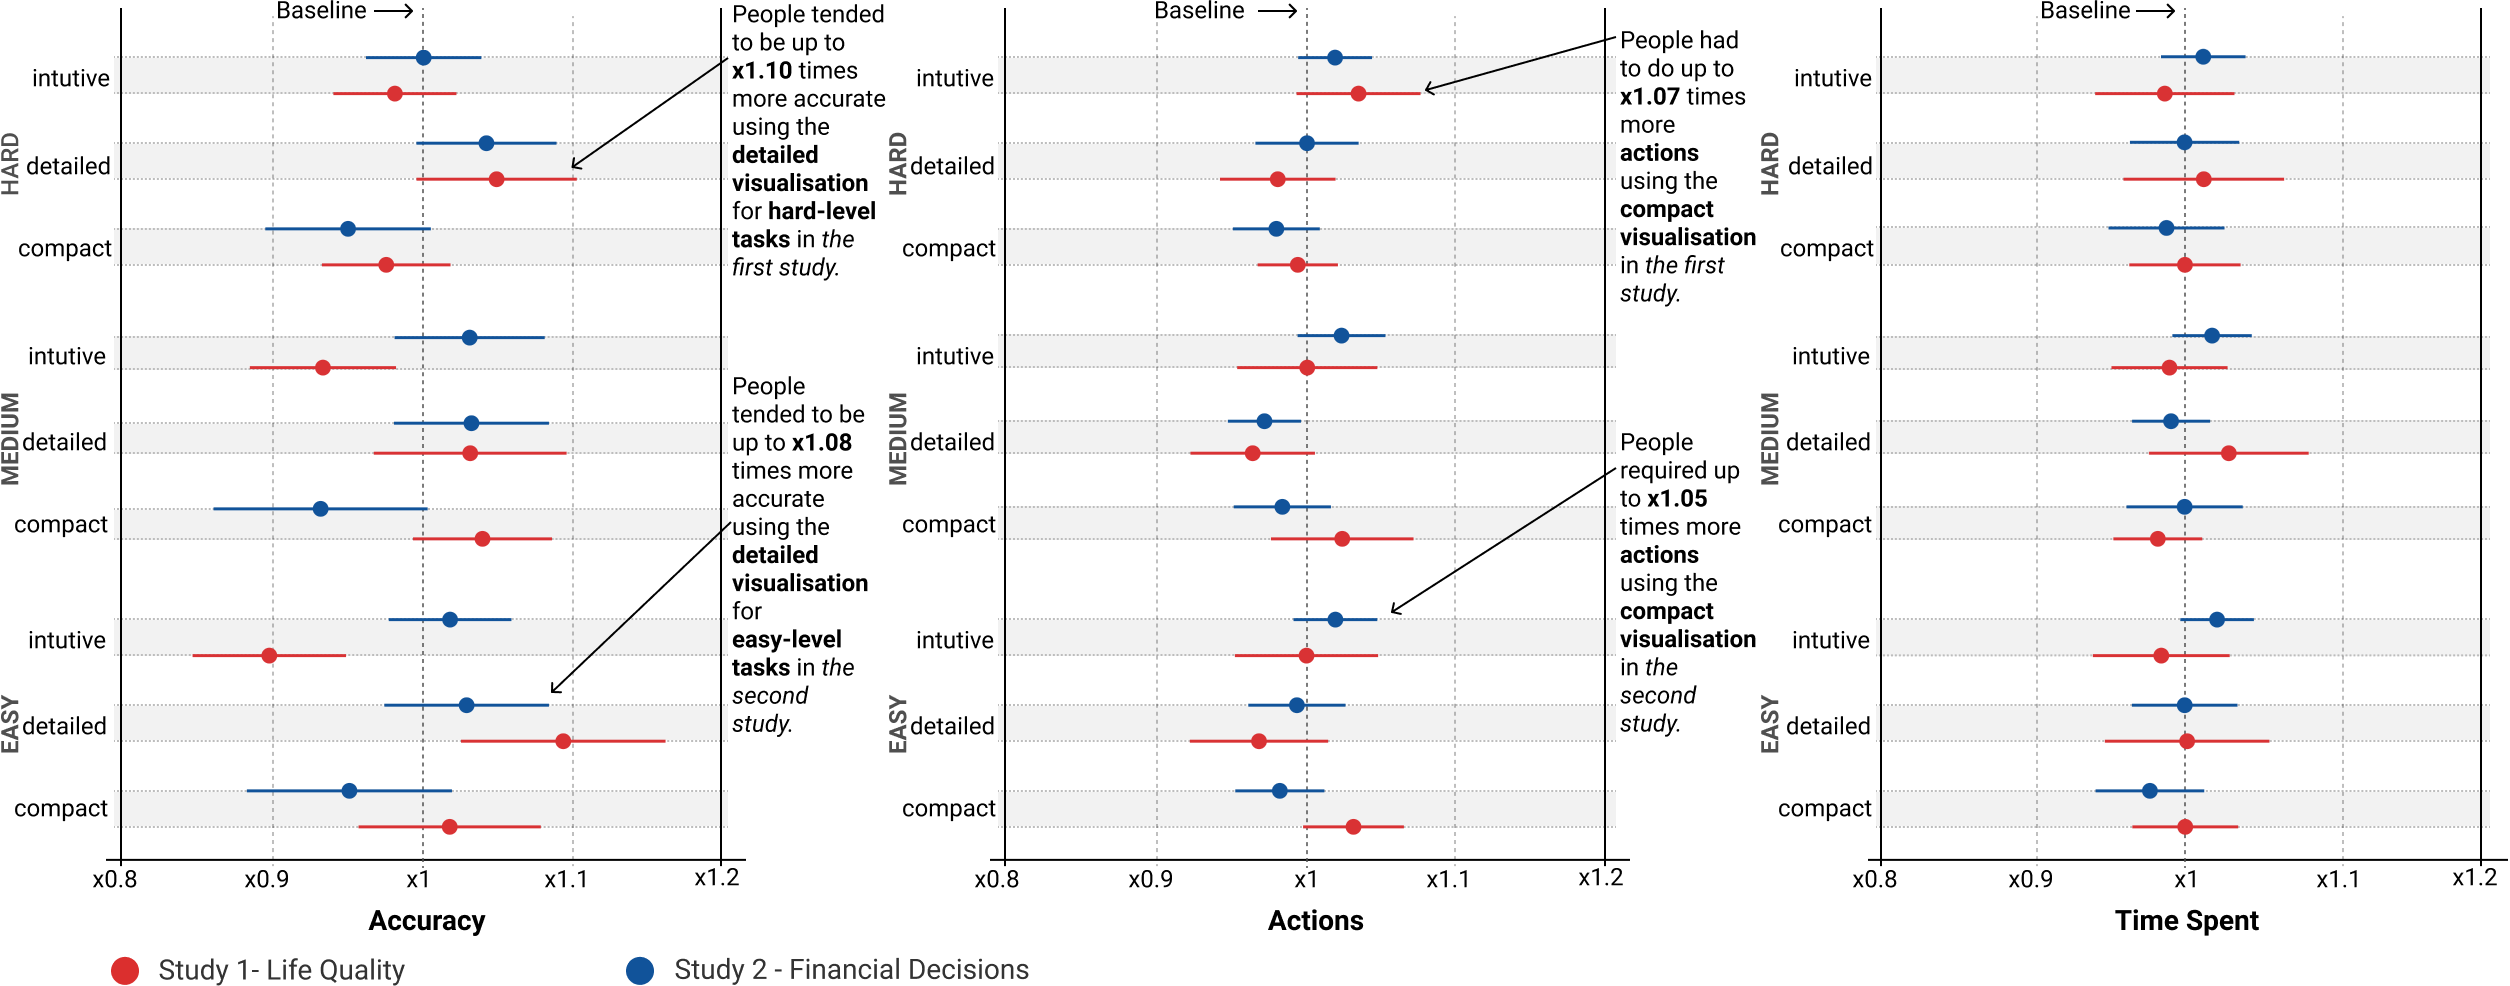
\includegraphics[width=\textwidth]{figures/studyCI_both.png}
\caption{Differences in variance for participants in the first and the second study with 95\% CI.}
\label{vizFigures3}
\end{figure*} 


\subsection{Accuracy}
In general participants tended to be more accurate using the \emph{detailed visualisation}. They were between 1.02 and 1.16 times more accurate for easy-level tasks, between 0.97 and 1.09 times for medium-level tasks, and between 1.00 and 1.10 times more accurate for hard-level tasks compared to the baseline. This tendency was replicated in the second study, where they were between 0.97 and 1.08 times more accurate for easy-level tasks, between 0.98 and 1.08 times for medium-level tasks, and between 1.00 and 1.09 times more accurate for hard-level tasks. 

Participants that used the \emph{compact visualisation} were not as accurate as participants that used the  \emph{detailed visualisation}.  In the second study the  \emph{compact visualisation} seemed to have a general negative impact in their accuracy. Participants were between 0.88 and 1.02 times accurate for easy-level tasks, between 0.86 and 1.00 times accurate for medium-level tasks and between 0.9 and 1.01 for hard-level tasks. In the first study, users struggled for hard level tasks where they performed poorly by being between 0.93 and 1.02 times accurate. However, in this study users tended to be between 0.96 and 1.08 times accurate for easy and between 0.99 and 1.08 for medium tasks. Because we got contradictory results in the studies, the results are not conclusive. However, participants tended to have a decremental performance for hard-level tasks in both studies, more specifically they were between 0.90 and 1.01 times accurate. 

Participants of the first study that used the \emph{intuitive} visualisation were in general less accurate. They were between 0.84 and 0.95 times accurate for easy-level tasks, between 0.88 and 0.98 times accurate for medium-level tasks and between 0.94 and 1.02 times accurate for hard-level tasks. In the first study, we used a map in combination with Chernoff-faces as intuitive representation. In the second study users were between 0.98 and 1.06 times accurate for easy, between 0.98 and 1.08 times for medium-level and between 0.96 and 1.04 times accurate for hard-level tasks using the \emph{intuitive} visualisation recommended by the financial expert. 

\subsection{Actions}

In the first study participants required the least actions for solving tasks using the \emph{detailed visualisation}. They required between 0.92 and 1.01 times actions for completing easy and medium-level tasks, and between 0.94 and 1.01 less actions for hard-level tasks. In the second study we observed a tendency of participants to require between 0.95 and 1.00 actions for finishing medium-level tasks confirming our observations in the first study. However, results for easy and hard-level tasks the results differed in the second study, where participants tended to show no effect when compared to the baseline. 

In the second study participants that used the \emph{intuitive} visualisation required between 0.99 and 1.05 actions for easy-level and between 1.00 and 1.06 for medium-level tasks. However, in the first study no significant differences were found for easy and medium-levels compared to the baseline. On the other hand for hard-level tasks, participants showed a tendency to require between 0.99 to 1.07 times actions to finish the tasks in the first study and between 0.99 and 1.04 in the seconds.

When using the \emph{compact visualisation} participants in the first study required between 1.00 and 1.06 times more actions for easy-level and between 0.98 and 1.07 for medium-level tasks. In contrast, they required between to 0.95 and 1.01 for easy and hard-level tasks and between 0.96 and 1.02 times actions for medium-level tasks. Despite of the results for easy and medium-level tasks, we observed that for hard-level tasks participants required between 0.96 and 1.02 times actions.

% Moving subjective stuff to the other section...


\subsection{Time}
In general no significant differences were found. The results indicate that in most cases the visualisations had no effect on how much time the participants spent when solving the tasks with the visualisations. In the first study we observed that participants that used the \emph{intuitive} visualisation tended to spend between 0.94 and 1.03 times more time than the baseline. In contrast, during the second study participants tended to spend between 0.98 and 1.04 more time to finish the tasks. 

In the first study, participants with the \emph{compact visualisation} showed no effect for easy and hard-level tasks, but they tended to spend between 0.95 and 1.01 time for medium-level tasks. In contrast, in the second study, participants showed no effect for medium-level tasks, but they required between 0.94 and 1.01 time for easy-level and between 0.95 and 1.03 time for hard-level tasks.

Participants of the first study showed no effect for easy tasks with the \emph{detailed} visualisation, but in general they spent between 0.98 and 1.08 time for medium, and between 0.96 and 1.07 for hard-level tasks. In contrast during the second study participants showed no effect for easy and hard-level tasks, but they showed a tendency to require between 0.96  and 1.01 time for medium-level tasks.

The time spent by users in the tasks could be affected by the selected evaluation platform. In \emph{Amazon Mechanical Turk} some users tend to pressure themselves towards finishing the HIT \citep{Paolacci2010}. Even though we considered this for the two studies, participants had 45 minutes to finish the evaluation and were informed that it would take 20 minutes on average. Results indicate that further exploration is required in this regard.

\def\arraystretch{1.5}
\begin{table}
  \centering
  \caption{Recommendations for each visualisation based in the results of subjective data in the two studies.}
    \begin{tabular}{l c c c }
    & \textbf{Intuitive} & \textbf{Detailed} & \textbf{Compact} \\ 
    \hline
    Visual appeal   &\checkmark&-&\checkmark \\
    Ease of use     &\checkmark&-&- \\
    Suitability     &-&\checkmark&\checkmark \\
    Liked it        &\checkmark&\checkmark&- \\
    Tasks were easy &\checkmark&\checkmark&- \\
    \hline
    Trust           &\checkmark&-&- \\
    Confidence      &\checkmark&-&- \\
    Credibility     &\checkmark&-&\checkmark \\
    Understanding   &\checkmark&-&\checkmark \\
    Accuracy representation &\checkmark&\checkmark&\checkmark \\
    \hline
    \multicolumn{4}{c}{\footnotesize{ \checkmark Recommended; - Not Conclusive;}}\\
    \end{tabular}%
  \label{tab:subjective}%
\end{table}%

\subsection{Subjective feedback}

In this section we summarize the results from subjective feedback. We provide recommendations based in our observations from the two studies in table \ref{tab:subjective}. 

\textbf{Intuitive visualisation:} In the first study participants agreed with the visualisation visual appeal $(Mdn = 4)$. However, they rated it with a low score $(Mdn = 3)$ for suitability, trust, confidence, credibility and understanding. We paid special attention when users mentioned the visualisation made the tasks look more difficult $(Mdn = 2.5)$. In contrast in the second study, after a better selection of the  visualisation, participants thoughts were more positive. Participants indicated the tasks seemed more easy to use $(Mdn = 5)$ and the visualisation was easy to understand $(Mdn = 5)$. The improved results in the second study indicate that a careful selection of the visualisation has a major impact in users trust and confidence in the visualisation.

\textbf{Detailed visualisation:} According to their posterior feedback, participants agreed in both studies that tasks felt easy to solve $(Mdn = 4)$ and in general they tended to like it $(Mdn = 4)$. They also agreed that the representation of accuracy was clear in the visualisation $(Mdn = 4)$. When comparing the results from the two studies, we can't give a recommendation about trust, confidence or credibility, since participants tended to be more positive in the second study $(Mdn = 4)$ but tended to be more conservative with their answers in the first study $(Mdn = 3)$. 

\textbf{Compact visualisation:} In both studies participants showed a positive attitude towards credibility, understanding and accuracy representation of the visualisation $(Mdn = 4)$. However some factors like trust and confidence were rated more conservatively $(Mdn = 3)$ and so no recommendations can be made towards these factors. However participants tended to think the visualisation was suitable for solving the tasks in the two studies and it was visually appealing $(Mdn = 4)$. 

\begin{figure*}[t]
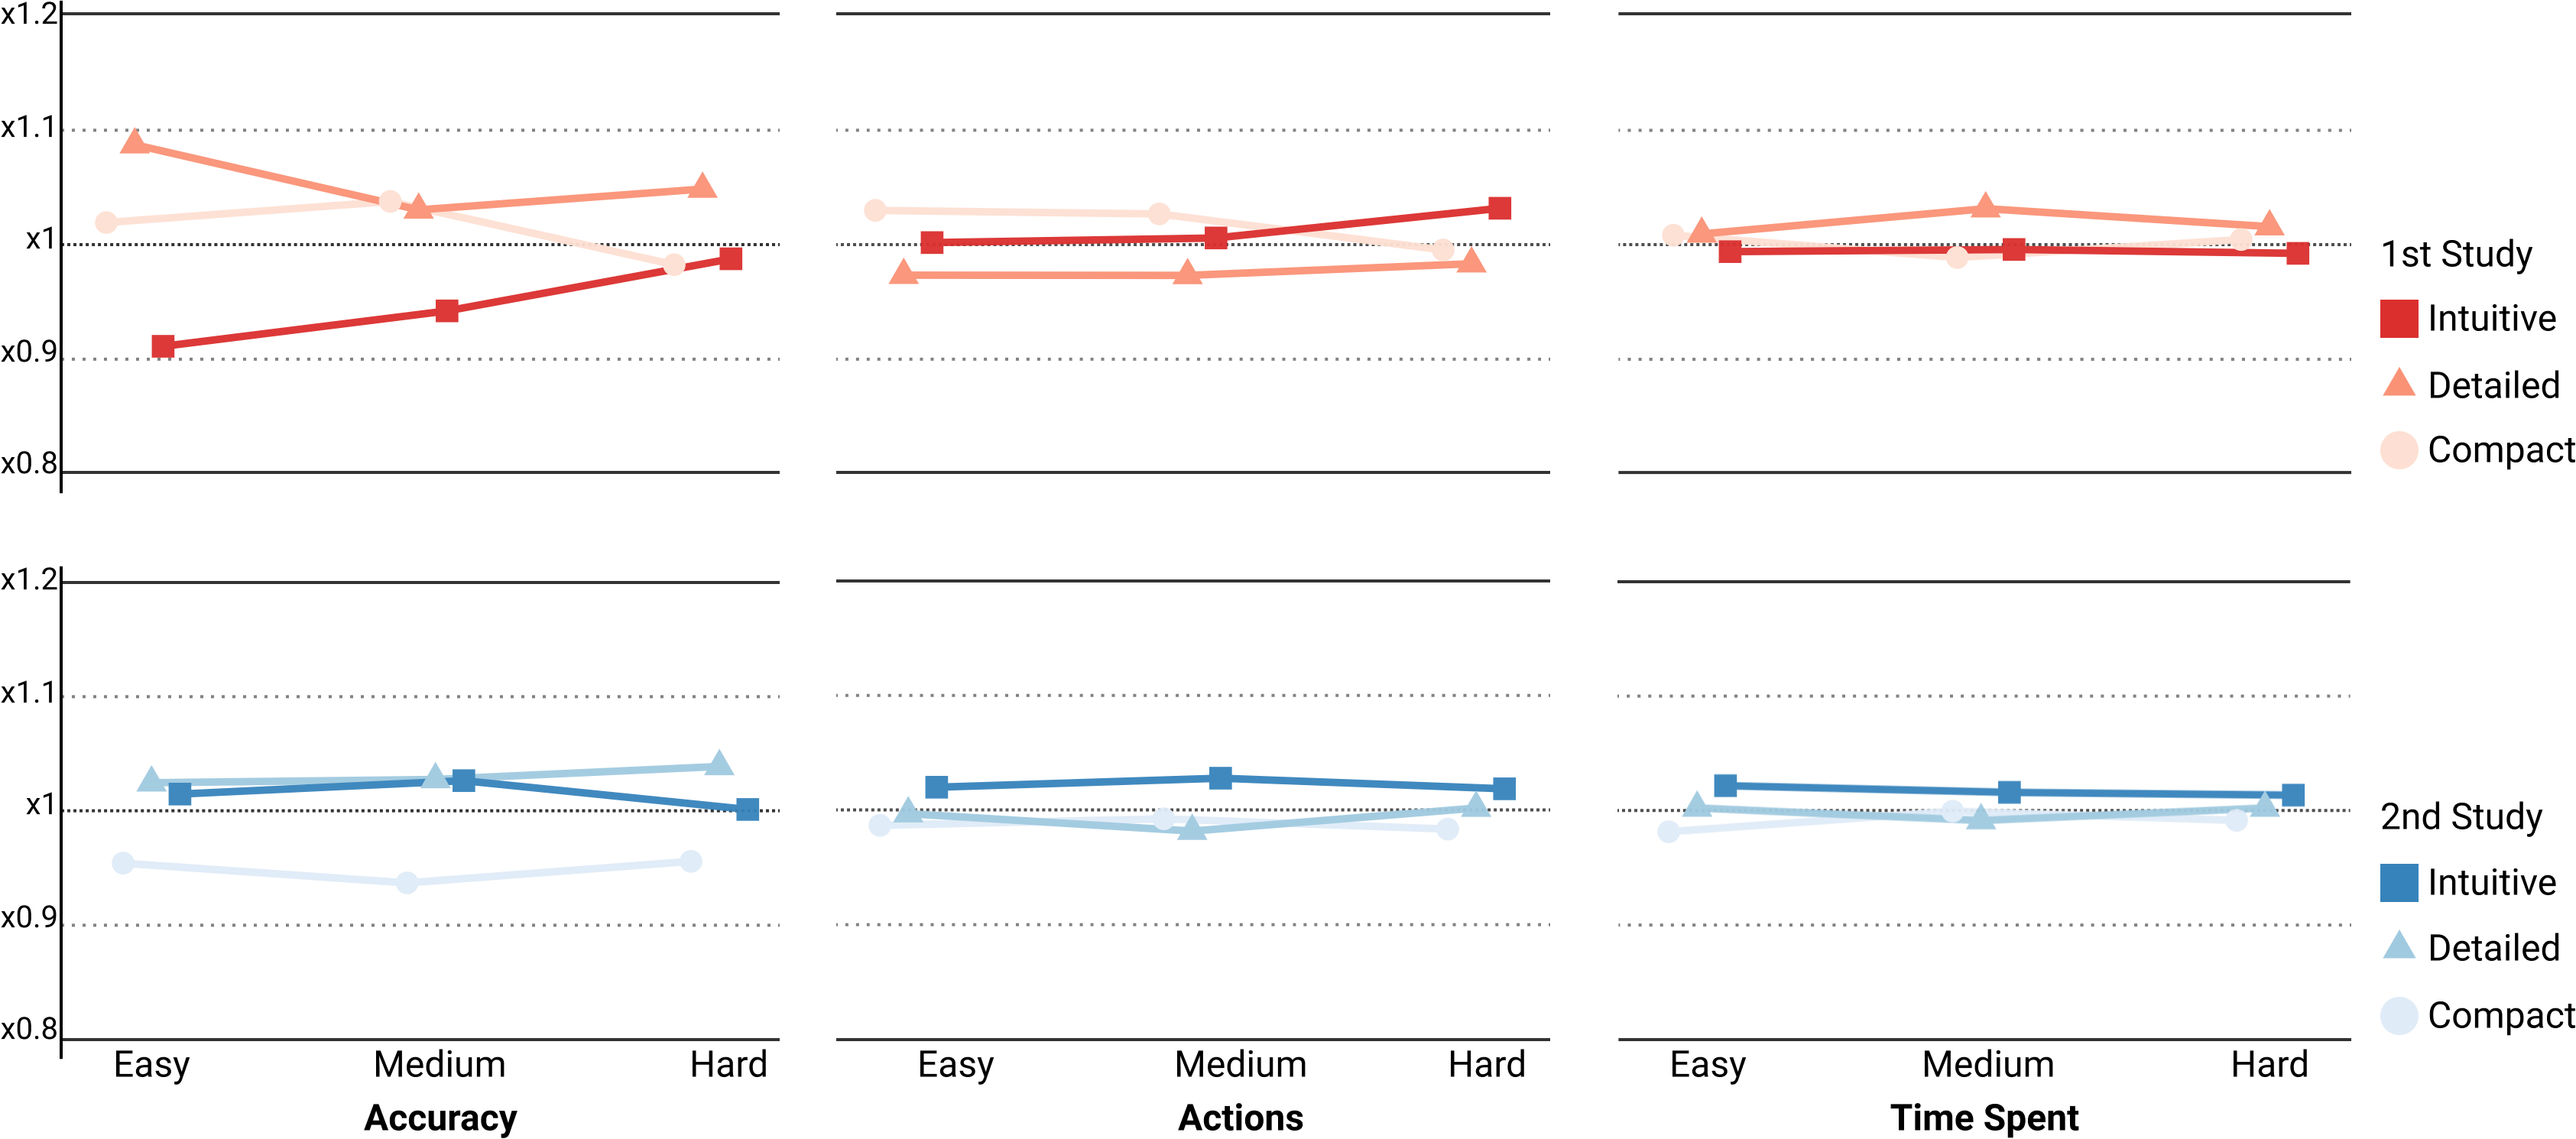
\includegraphics[width=\textwidth]{figures/question2.png}
\caption{Left to right: Differences compared to the baseline, for accuracy, actions and time spent in first and second studies, grouped by level of difficulty.}
\label{question2}
\end{figure*} 

\section{Answering the research questions} % (fold)
\label{sub:researchquestions}

\emph{1. Regarding criteria such as speed, accuracy, usability, and uncertainty, what are the benefits and challenges of intuitive, detailed, and compact visualisations in an interactive decision-making process?}

The \textbf{intuitive visualisation} is a good option when precision is required for easy and medium tasks. Users seem to understand and have confidence with the visualisation. One of the main challenges is the suitability of the visualisation to the context. Our two studies demonstrate that the selection of a good visualisation has a major impact in usability and uncertainty factors.

The \textbf{detailed visualisation} offers improved accuracy for all levels of difficulty. Users tended to require less actions than the average to finish the tasks. Regarding usability, users tended to find the visualisation suitable, and they liked it. Regarding uncertainty users thought that the accuracy representation was clear. The challenge about the detailed visualisation is around the uncertainty metrics, participants showed a neutral attitude about their confidence, trust and credibility in the two studies. Also the visual appeal and ease of use. Further analysis is required regarding these aspects.

The \textbf{compact visualisation} had mixed results about accuracy and actions. While not conclusions can be made about these factors, participants tended to show positive attitudes towards uncertainty. They found the visualisation credible, understandable and thought that the accuracy representation was clear. Further exploration about the compact visualisation is required.


\emph{2. How do the visualisations' performance measures accuracy, actions, and time spent relate to task difficulty?}

In figure \ref{question2} we illustrate the differences in performance for accuracy, actions and time spent grouped by level of difficulty of the tasks.

The \textbf{detailed visualisation} excelled in all levels of difficulty for accuracy and medium-level actions. Users were more accurate in general and tended to perform the least actions when solving the tasks. According to participants feedback, this visualisation felt suitable for solving the tasks and made them look easy to solve. However, no conclusions can be made in how much time the users spent with the visualisation in comparison to others. 

Based on the results of the two studies we conclude that an \textbf{intuitive visualisation} works better for easy and medium-level tasks. However, to achieve that level of accuracy participants required to do more actions to finish the tasks. We came to these conclusions after a poor performance with the Chernoff-Faces visualisation in the first study. On the other hand, in the second study, participants reported more confidence, and praised the visualisation for its ease of use, confidence and understanding, reflecting these factors in their performance.

Mixed results were found with the \textbf{compact visualisation}. In the first study users demonstrated a better accuracy for easy and medium tasks, but tended to require more actions. In contrast, during the second study, participants were in general less accurate in the three difficulty levels. Participants required more actions to finish the tasks. For hard-level tasks users were less accurate in the two studies but still required less actions to finish their tasks.

\def\arraystretch{1.5}
\begin{table*}
  \centering
  \caption{Recommendations based in the results observed in the two studies, grouped by visualisation and level of difficulty.}
    \begin{tabular}{p{0.25\linewidth} c c c | c c c | c c c }
    & \multicolumn{3}{c}{\textbf{Intuitive}} & \multicolumn{3}{c}{\textbf{Detailed}} & \multicolumn{3}{c}{\textbf{Compact}} \\ 
    \hline
    & easy & medium & hard & easy & medium & hard & easy & medium & hard \\
    \hline
    \textbf{Accuracy} is an important factor in the task.    &\checkmark&\checkmark&-&\checkmark&\checkmark&\checkmark&-&-&\times \\
    Number of \textbf{actions} is an important factor in the task. &-&-&\times&-&\checkmark&-&-&-&\checkmark \\
    \textbf{Time spent} is an important factor in the task.  &-&-&-&-&-&-&-&-&-\\
    \hline
    \multicolumn{10}{c}{\footnotesize{ \checkmark Recommended; - Not Conclusive; $\times$ Not Recommended;}}\\
    \end{tabular}%
  \label{tab:recommendations}%
\end{table*}%

\section{Recommendations for Implementation} % (fold)
\label{sub:recommendations}

Visualisation for non-expert users requires a careful measurement of qualities and level of difficulty to solve a problem. Modern technologies like immersive analytics \citep{Bonada2016}, demand that the choice of the visualisation should be progressively adapted to the complexity of the task as required. We believe  the communication of uncertainty is essential in the decision-making, and should be integrated as part of the core in any visualisation presented to the users. We would like to give the following recommendations for visual analytics applications aimed to non-expert users based on our findings, results are summarized in table \ref{tab:recommendations}.

\textbf{Detailed  visualisation:} We can recommend the use of this visualisation for all levels of difficulty. However, one of the potential drawbacks a designer could face during implementation is the responsiveness of the visualisation in small screens. Even though users required to perform less actions, a detailed visualisation would shine in larger spaces, where users can manipulate the variables and inspect the details as the information reactively changes. Detailed visualisation could be saved to be used for harder-level tasks, while using intuitive or compact visualisations to illustrate easy and medium-level tasks.

\textbf{Intuitive visualisation:} Our recommendation for implementation is that the designer has to be careful with the selection of an intuitive visualisation, because even if a visualisation receives positive comments regarding its appeal, it is worth doing a deep analysis in other aspects such as confidence, trust and credibility. Given that according to our studies, these decisions can dramatically affect the performance of users in all levels of difficulty.

\textbf{Compact visualisation:} We cannot give a recommendation for easy and medium-level tasks and we suggest to not use a compact visualisation when accuracy is a critical factor for hard level-tasks. A compact visualisation, like the dotplot presented by \citep{kay_when_2016}, has potential because it can show clearly a deep insight towards uncertainty while requiring less actions to achieve a task. According to participant's feedback, the visualisation was credible, and understandable, but they were not sure when asked about their trust or confidence. Further research is required about the effects of a compact visualisation in the decision making for VA applications.



\section{Conclusion} % (fold)
\label{sec:conclusion}
% =============================================================================

%%% Work in progress..

Exploring the challenges of VA for non-experts is a growing research field \citep{kwon2011visual}. While advice on mapping types of data to an ideal representation does exist \citep{Wongsuphasawat2016}, information about different visualisations' qualitative and quantitative performance in an interactive decision-making process for non-experts does not. To address this research gap, we have examined the suitability of intuitive, compact, and detailed visualisations in the risk-based decision-making process for non-experts in an application facilitating the exploration of variables involved in a prediction model. By allowing the users to interactively change the importance of different variables, users could steer an algorithm predicting these aspects from a dataset.

Using objective and subjective means proposed by earlier work, we determined the benefits and trade-offs of these visualisations for different difficulty levels. We found that while a intuitive visualisation can be a good choice for easy-level and medium-level tasks, hard-level tasks are best supported with a richer, yet visually more demanding visualisation, potentially at the cost of some usability aspects. 

Our research extends previous work on the challenges of supporting non-experts with VA: \cite{kwon2011visual} reported a set of \q{roadblocks} inhibiting non-experts from successfully using popular VA applications. As these are commonly built for experts, their utility can be \q{unreachable} to non-experts due to their limited domain experience, low graph literacy, and inaccurate mental model. Therefore, if we want to extend the user-base of VA to this user group, we may have to take a step back from these highly specialised and powerful applications. Instead, this endeavour may call for a new generation of applications that are closely tied to a user's abilities, preferences, and the difficulty of the problem to be solved. \cite{huang2015personal} explored the challenges of personal VA and suggested that an application that is to be successful in this field needs to consider a user's context and provide \q{appropriate baselines to support reasoning about data}.

Our work presents a first step towards providing such a baseline: Defining Huang et al.'s user context as the difficulty of the problem to be solved or level of insight to be gained, we have evaluated the adequacy of a certain visualisation for supporting the VA process of non-experts. Following Shneiderman's visual information seeking mantra \citep{shneiderman1996} of increasing information density as required, we suggest increasing complexity and capability of a model's representation as the task difficulty and required level of insight increase.

Our results and those of \cite{kwon2011visual} have indicated that confronting non-experts with a powerful, but unnecessary complex visualisation is detrimental to solving simple problems. Instead, we found that by adapting the visualisation to the difficulty of the task, a favourable balance may be struck between various objective and subjective aspects, and the decision-making process optimally supported. While experts know which view to choose, non-experts do not \citep{kwon2011visual}. By defining strengths and weaknesses of three visualisation types for problems of varying difficulty, we provided a first step towards the definition of a set of visualisations that may be chosen to support the growing group of non-expert users.


% and clearly determine what visualisation may be most adequate for a certain level of insight-gaining to solve a problem Our: first step. havve dtermined the right view (roadbloack) and thereby gained an insight into how we can best support non-experts with a VA application.

% Adapt Mantra to ourt findings
% Simple and lcear first, with increasing complexity and capavilities as the required insight level increases

% An expert knows what view to choose [cite] whereas laymen struggle with this complexity.
% Intro: Uswers encounter road blocks, [cite], 
% Therfore,app needs to consider limited experience and consider context == adapted to task!
% -- gradually increase complexity/capbilities of vis as the problem level rises!!!!
% -- adaptive visulisation to problem? Deffo to user, cite [xxx]

% To circumvent roadbloacks, we need adaptive visualisation based on required levwel of insight. Can be formulated?
% Only if machine knows user intent

% The roadbloack reported by [cite xxx] suggest that while the work in VA has been focussed on experts, the resulting applications/visualisations have become ``unreachable'' for non-experet users. They struggle to understand these and .... etc.
% As XXX state, VA systems for non-expers need to adapt to their limited 

% To make VA mor accessible to non-experts, we have examined the benefits and challenges of..
% Need for adaptive...
% An ``appropriate baseline'' here is the close match of insight level needed and optimal visualisation, needs to happen dynamically. For this process our works provides baisc guidance that shows pros/cons of 3 visualisation types in the decision-making process for laymen.

% Non-expert challneges
% - Prev work (cite xxx journal) : limited insight, roadblocks due to high difficulty,
% >> same here: low precision on more difficult tasks (but still notable differences between visualisations).

% section conclusion (end)


\subsection{Limitations and Future Work} % (fold)
\label{sub:limitations}
% =============================================================================
While previous work has shown the suitability of AMT for conducting user studies in the visualisation domain \citep{heer2010crowdsourcing, yang_understand_2014}, results should be interpreted with caution, as studies were unsupervised. However, online studies are common and we hope that the measures described in section \emph{Main Study} have sufficed to ensure data validity. Further, users were guided by the questions to facilitate evaluation, and only a limited number of risks (four) was used to simplify the application while allowing decision-making with three or more parameters (high-level insights \citep{yang_understand_2014}). To avoid ``roadblocks'' \citep{kwon2011visual}, we used a mixture of confirmatory and exploratory analyses. 

With benefits and challenges of the three visualisations established, future work will examine performance in a purely exploratory environment and whether findings are applicable to other domains. An extension to other fields would allow researchers to investigate whether our findings and recommendations are domain-specific, or may hold a greater validity. Yet, this goes beyond the scope of this journal and may thus serve as inspiration for the community.


% - visualisations not optimised, so none has advantage.
% This is a foundational study regarding \emph{type} of visualisation that is best suited to present data and prediction results based on user input



% section limitations (end)

%% The Appendices part is started with the command \appendix;
%% appendix sections are then done as normal sections
%% \appendix

%% \section{}
%% \label{}

%% If you have bibdatabase file and want bibtex to generate the
%% bibitems, please use
%%
\section*{Acknowledgements}
Katrien Verbert is a postdoctoral fellow of the Research Foundation Flanders (FWO).

\section*{References}
  \bibliographystyle{elsarticle-harv} 
  \bibliography{mybibfile}

%% else use the following coding to input the bibitems directly in the
%% TeX file.

%\begin{thebibliography}{00}

%% \bibitem[Author(year)]{label}
%% Text of bibliographic item

%\bibitem[ ()]{}

%\end{thebibliography}
\end{document}

\endinput
%%
%% End of file `elsarticle-template-harv.tex'.
